\documentclass{article}

\PassOptionsToPackage{numbers,sort&compress}{natbib}
\usepackage[preprint]{../../neurips}
\usepackage[utf8]{inputenc}
\usepackage[T1]{fontenc}
\usepackage{hyperref}
\usepackage{url}
\usepackage{booktabs}
\usepackage{microtype}
\usepackage{xcolor}
\usepackage{graphicx}
\usepackage{subcaption}
\usepackage{multirow}
\usepackage{array}
\usepackage{adjustbox}
\usepackage{enumitem}
\usepackage{algorithm}
\usepackage{algpseudocode}
\usepackage{amsmath}
\usepackage{amssymb}
\usepackage{amsfonts}
\usepackage{amsthm}
\usepackage{mathtools}
\usepackage{bm}

\title{CDA: Post-hoc Domain Generalization by Seeking Distributional Canalization}
\author{Anonymous Authors}

\newtheorem{theorem}{Theorem}[section]
\newtheorem{proposition}[theorem]{Proposition}
\newtheorem{lemma}[theorem]{Lemma}
\newtheorem{corollary}[theorem]{Corollary}
\newtheorem{assumption}[theorem]{Assumption}
\theoremstyle{definition}
\newtheorem{definition}[theorem]{Definition}
\newtheorem{remark}[theorem]{Remark}

\newcommand{\RR}{\mathbb{R}}
\newcommand{\EE}{\mathbb{E}}
\newcommand{\cC}{\mathcal{C}}
\newcommand{\cA}{\mathcal{A}}
\newcommand{\cV}{\mathcal{V}}
\newcommand{\cU}{\mathcal{U}}
\newcommand{\argmin}{\operatorname*{arg\,min}}
\newcommand{\argmax}{\operatorname*{arg\,max}}
\newcommand{\Cov}{\operatorname{Cov}}
\newcommand{\Var}{\operatorname{Var}}
\newcommand{\tr}{\operatorname{tr}}
\newcommand{\proj}{\operatorname{Proj}}
\newcommand{\TBD}{\textbf{TBD}}
\newcommand{\Expected}[1]{\textcolor{gray!75!black}{\emph{#1}}}
\newcommand{\cda}{\textup{\textsc{CDA}}}
\newcommand{\swad}{\textup{\textsc{SWAD}}}
\newcommand{\diwa}{\textup{\textsc{DiWA}}}
\newcommand{\eoa}{\textup{\textsc{EoA}}}
\newcommand{\erm}{\textup{\textsc{ERM}}}
\newcommand{\ood}{\textup{\textsc{OOD}}}
\newcommand{\one}{\mathbf{1}}
\newcommand{\simplex}{\Delta}
\newcommand{\norm}[1]{\left\lVert #1 \right\rVert}
\newcommand{\abs}[1]{\left\lvert #1 \right\rvert}
\newcommand{\inner}[2]{\left\langle #1, #2 \right\rangle}
\newcommand{\paren}[1]{\left( #1 \right)}
\newcommand{\braces}[1]{\left\{ #1 \right\}}
\newcommand{\thetaw}{\bar{\theta}(w)}
\newcommand{\ub}{u_E}

\begin{document}

\maketitle

\begin{abstract}
Current post-hoc domain generalization methods are usually justified by parameter-space flatness, diversity among models being averaged, or plain validation performance. We study \emph{distributional canalization}, namely source-mixture sensitivity, as a source-only post-hoc criterion for evaluating deployable models. Our central theoretical claim has two parts. First, under a source-supported hidden-shift model, target risk is upper bounded by mean source risk plus a source-mixture sensitivity term, so minima with low sensitivity to small redistributions of source-support mass are more generalizable in that regime. Second, expanding that objective on a checkpoint family yields a practical surrogate that leads directly to \cda{}, a checkpoint-soup method built from worst-domain source fit, an interaction-based hidden-shift penalty, and a mergeability term. The theorem-bearing contribution is organized around a model-level local tangent-space ambiguity set over source mixtures, not around soups themselves. We prove the target-risk bound, an exact closed form for the associated hidden-shift robust risk in the tangent model, variance and interaction decompositions that expose complementarity and redundancy, a sufficient low-curvature regime explaining why flatness works, and a constructive example showing why pooled flatness can miss source-mixture sensitivity. For the practical weighting problem on a fixed checkpoint family, we prove convexity, projected-subgradient convergence, and a conditional predictive-mixture-to-single-soup transfer bound controlled by a mergeability remainder. New \cda{} empirical results remain intentionally marked \TBD{}, while published benchmark context from prior post-hoc domain generalization papers is included to define the target bar.
\end{abstract}

\section{Introduction}

Post-hoc domain generalization matters because it is one of the few robustness strategies that can be attached to a strong empirical-risk-minimization pipeline without retraining. A single training run produces a dense checkpoint bank, and one deployable model is chosen only after training has already finished. This regime is operationally attractive and empirically credible. On DomainBed, \swad{} reported an average accuracy of \(66.9\) across PACS, VLCS, OfficeHome, TerraIncognita, and DomainNet, improving \erm{} from \(63.3\) \citep{cha2021swad}. Later weight-averaging work pushed the frontier higher, including \diwa{}, whose strongest published linear-probe setting reports \(68.0\) average accuracy \citep{rame2022diwa}. The practical question is therefore no longer whether post-hoc averaging can help. The unresolved question is \emph{what criterion the final post-hoc model should optimize}.

The dominant explanation in this niche is flatness. \swad{} states that finding flat minima reduces the domain generalization gap \citep{cha2021swad}. That theory is important, but it is incomplete in two ways. First, flatness mainly explains why averaging may be \emph{safe}; it does not fully explain why some averaged solutions are more \emph{useful} than others. Second, later work has emphasized that locality and diversity matter jointly under shift. \diwa{} explicitly frames weight averaging through a bias-variance-covariance-locality decomposition and argues that good \ood{} averaging requires a trade-off between diversity and locality \citep{rame2022diwa}. These are not competing stories. They can be interpreted through a common source-side robustness lens.

This paper studies the following source-side post-hoc criterion:
\begin{quote}
\textbf{Distributional canalization.} A model is preferable when its source performance is stable under small local redistributions of source support mass.
\end{quote}

The claim is intentionally not specific to soups. It is a statement about models, weights, and minima. Soups enter only later, as one practical way to search for models with low source-mixture sensitivity using a completed checkpoint bank.

The intuition is direct. In post-hoc DG, the target domain is unavailable, but source data still contain latent heterogeneity. A future shift can be approximated locally as a nearby change in the mixture of source environments or source slices. A model is therefore desirable when its loss does not change much under those small redistributions. This object lives in \emph{distribution space}, not parameter space. Flatness becomes a sufficient but not necessary mechanism: if nearby parameter perturbations barely alter the domain-loss vector, then source-mixture sensitivity is small, but the converse need not hold.

This perspective yields a two-step story. First, we show that under a source-supported hidden-shift assumption, target risk is controlled by mean source loss plus source-mixture sensitivity. Second, starting from a checkpoint bank, we derive a practical soup method by expanding that objective into terms that are estimable and optimizable:
\begin{itemize}[leftmargin=1.3em]
    \item \textbf{source-fit}, from the target-risk bound itself;
    \item \textbf{hidden-shift sensitivity}, because the final predictor should be canalized against local redistributions of source mass; and
    \item \textbf{mergeability}, because the predictive mixture being optimized must still transfer to one actual deployable soup.
\end{itemize}
One practical surrogate method, \cda{}, solves a checkpoint-family approximation to that objective after strengthening the source-fit term to worst-domain risk and replacing the exact canalization term by a quadratic interaction surrogate.

The paper makes five contributions.
\begin{enumerate}[leftmargin=1.4em]
    \item We formalize \emph{distributional canalization} as a source-side post-hoc robustness criterion and prove that, under a source-supported hidden-shift model, target risk is upper bounded by mean source risk plus source-mixture sensitivity.
    \item We prove an exact local ambiguity-set identity for hidden-shift robust source risk and derive variance and pairwise-interaction decompositions that make complementarity mathematically explicit.
    \item We prove a sufficient low-curvature corollary showing why flat minima can help under this criterion and a constructive separation theorem showing why pooled flatness is not enough by itself.
    \item We derive \cda{} as a practical surrogate implementation over a checkpoint bank by expanding the canalization objective into source-fit, interaction, and mergeability terms, and we prove convexity, projected-subgradient convergence, and a conditional predictive-mixture-to-single-soup transfer bound.
    \item We provide a complete NeurIPS-style manuscript with analytical figures, a published benchmark context table, and a \TBD{}-only section for all new \cda{} experiments.
\end{enumerate}

\begin{remark}
This paper does \emph{not} claim that distributional canalization fully explains all successful averaging methods, nor that \cda{} must dominate every post-hoc baseline on every benchmark. The strongest honest claim is narrower: source-mixture sensitivity is a useful post-hoc criterion under which flatness appears as a useful special case, and \cda{} is a practical surrogate for optimizing that criterion on a checkpoint bank.
\end{remark}

\begin{figure}[t]
    \centering
    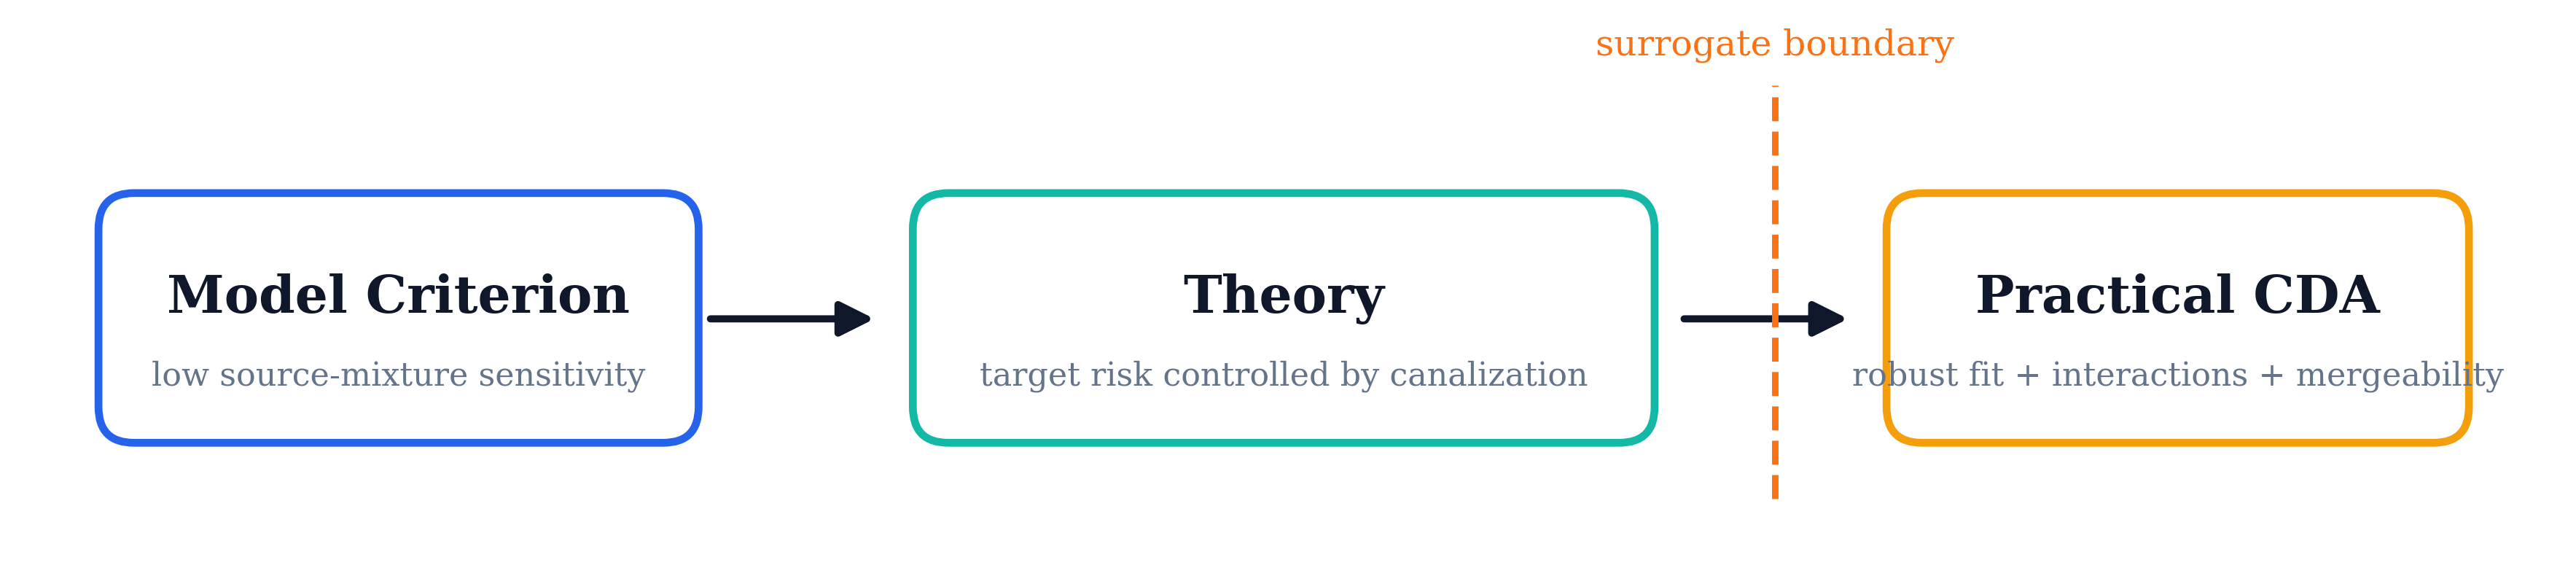
\includegraphics[width=\linewidth]{figures/cda_overview.png}
    \caption{\textbf{Two-part structure of the paper.} Left: the theorem-bearing object is model-level source-mixture sensitivity under a local tangent perturbation model, which yields a target-risk upper bound under source-supported hidden shift. Right: on a completed checkpoint bank, \cda{} is the operational surrogate obtained by expanding that objective and replacing it with worst-domain source fit, an interaction-based hidden-shift term, and a mergeability penalty.}
    \label{fig:overview}
\end{figure}

\section{Related Work}

\paragraph{Post-hoc domain generalization.}
DomainBed established that carefully tuned baselines remain difficult to beat under controlled evaluation \citep{gulrajani2021domainbed}. In that setting, post-hoc methods are attractive because they preserve the original training pipeline. \swad{} made this niche serious by showing strong gains from dense checkpoint averaging \citep{cha2021swad}. \eoa{} further showed that averaging can improve model selection and performance in domain generalization \citep{arpit2021ensemble}. These methods establish that the final deployable predictor is often not the last checkpoint.

\paragraph{Flatness, diversity, and weight averaging.}
\swad{} justifies post-hoc DG through flat minima \citep{cha2021swad}. \diwa{} broadens that picture by emphasizing diversity and locality jointly \citep{rame2022diwa}. Model soups and mode-connectivity work explain why averaging is viable when models lie in a common compatible region \citep{garipov2018fge,frankle2020linear,wortsman2022soups}. We do not dispute these observations. We treat them as partial views of a larger source-side robustness object.

\paragraph{Stability and data-distribution perturbations.}
Algorithmic stability links sensitivity to perturbations with generalization \citep{bousquet2002stability,hardt2016sgd}. Tangent Prop framed invariance through low derivatives along nuisance directions \citep{simard1991tangent}. Influence-function analyses and local DRO formalize sensitivity to example reweighting and nearby distributions \citep{koh2017influence,duchi2020variance,duchi2021learning}. Our paper pulls these ingredients into the post-hoc DG setting: the nuisance directions are not input transformations or arbitrary weight perturbations, but local redistributions of source-domain mass.

\paragraph{DG theory and robust source risk.}
The classical domain-adaptation theory of \citet{ben2010theory} clarifies that source-target divergence remains uncontrollable without target information. This is why a source-only post-hoc theory should focus on source-side quantities that can be optimized directly. Worst-domain source risk is one such quantity, and local hidden-shift sensitivity is another.

\section{Distributional Canalization}
\label{sec:canalization}

\subsection{Model-level setup}

We assume \(E\) labeled source domains with held-out validation splits
\[
\cV_e = \braces{z_{e,j}}_{j=1}^{n_e},
\qquad
z_{e,j}=(x_{e,j}, y_{e,j}),
\qquad
1 \le e \le E.
\]
For a model \(f_\theta\), let \(L_e(\theta)\) denote the source-domain validation risk on domain \(e\). Collect the domain losses into the vector
\[
L(\theta) = \paren{L_1(\theta),\dots,L_E(\theta)}^\top \in \RR^E,
\qquad
\bar L(\theta)=\frac{1}{E}\one^\top L(\theta).
\]
Let the nominal source mixture be uniform,
\[
\ub = \frac{1}{E}\one,
\]
and define the local tangent ambiguity set
\begin{equation}
\cA_\rho
:=
\braces{
\alpha=\ub+\delta :
\one^\top\delta=0,
\;
\norm{\delta}_2 \le \rho
},
\label{eq:ambiguity}
\end{equation}
This is the theorem-bearing local tangent approximation to nearby source-mixture redistributions. We do \emph{not} require \(\alpha\) to remain inside the simplex in the exact identity below; if one additionally enforces nonnegativity, the same closed form holds only in the sufficiently local regime where the maximizing perturbation remains feasible.
The \emph{distributional canalization score} of \(\theta\) is the local hidden-shift robust risk
\begin{equation}
\mathcal R_\rho(\theta)
:=
\sup_{\alpha\in \cA_\rho}
\alpha^\top L(\theta).
\label{eq:model_robust_risk}
\end{equation}

\begin{definition}[Source-mixture sensitivity]
\label{def:sensitivity}
The \emph{source-mixture sensitivity} of \(\theta\) at radius \(\rho\) is
\begin{equation}
\mathcal S_\rho(\theta)
:=
\mathcal R_\rho(\theta)-\bar L(\theta).
\label{eq:sensitivity}
\end{equation}
We call \(\theta\) \emph{\(\rho\)-canalized} when \(\mathcal S_\rho(\theta)\) is small.
\end{definition}

\subsection{Why low source-mixture sensitivity improves generalization}

\begin{assumption}[Source-supported hidden shift]
\label{ass:source_supported}
There exist a radius \(\rho\ge 0\) and an approximation constant \(\epsilon_{\mathrm{app}}\ge 0\) such that the target-domain risk satisfies
\begin{equation}
L_T(\theta)
\le
\alpha_T^\top L(\theta) + \epsilon_{\mathrm{app}}
\qquad
\text{for some } \alpha_T \in \cA_\rho
\label{eq:source_supported}
\end{equation}
for every \(\theta\) in the model family of interest.
\end{assumption}

Assumption~\ref{ass:source_supported} is the paper's explicit hidden-shift model. It says the unseen target behaves like a sufficiently local redistribution of source-domain mass, up to approximation error \(\epsilon_{\mathrm{app}}\).

\begin{theorem}[Target-risk control by distributional canalization]
\label{thm:target_control}
Under Assumption~\ref{ass:source_supported}, for every \(\theta\),
\begin{equation}
L_T(\theta)
\le
\mathcal R_\rho(\theta)+\epsilon_{\mathrm{app}}.
\label{eq:target_control_abstract}
\end{equation}
Consequently,
\begin{equation}
L_T(\theta)
\le
\bar L(\theta)+\rho \norm{P_\perp L(\theta)}_2+\epsilon_{\mathrm{app}}.
\label{eq:target_control_explicit}
\end{equation}
\end{theorem}

Theorem~\ref{thm:target_control} is the main answer to the paper's motivating question. Under a source-supported hidden shift, minima with low sensitivity to small redistributions of source-support mass have lower target risk. The rest of the paper explains why flatness can help under this criterion and how a practical checkpoint-soup algorithm arises from expanding the bound.

\subsection{Exact ambiguity identity}

Define the centering projection
\[
P_\perp := I - \frac{1}{E}\one\one^\top.
\]

\begin{proposition}[Exact local hidden-shift identity for the tangent model]
\label{prop:exact_identity}
Under the local tangent ambiguity set \(\cA_\rho\) of Eq.~\eqref{eq:ambiguity}, which imposes only the centered affine constraints \(\one^\top \delta = 0\) and \(\norm{\delta}_2 \le \rho\), for any \(\theta\),
\begin{equation}
\mathcal R_\rho(\theta)
=
\bar L(\theta) + \rho \norm{P_\perp L(\theta)}_2.
\label{eq:exact_identity}
\end{equation}
Equivalently,
\begin{equation}
\mathcal S_\rho(\theta)=\rho \norm{P_\perp L(\theta)}_2.
\label{eq:exact_sensitivity}
\end{equation}
\end{proposition}

Equation~\eqref{eq:exact_identity} is the paper's main expansion identity. It is not a heuristic penalty. It is the exact support function of the centered \(\ell_2\) tangent ambiguity set of Eq.~\eqref{eq:ambiguity}. If one additionally intersects \(\cA_\rho\) with the simplex, the same identity holds only in the sufficiently local regime where the maximizing perturbation remains nonnegative.

\begin{proposition}[Worst-domain risk as a robust prior]
\label{prop:worst_domain_prior}
For any \(\theta\),
\begin{equation}
\sup_{\pi \in \simplex^E} \pi^\top L(\theta)
=
\max_{1\le e\le E} L_e(\theta).
\label{eq:worst_domain_identity}
\end{equation}
\end{proposition}

Proposition~\ref{prop:worst_domain_prior} is trivial but important: the usual worst-domain objective is itself a robust prior over source environments. \cda{} combines that robust prior with the local hidden-shift sensitivity of Proposition~\ref{prop:exact_identity}.

\subsection{Variance and interaction decompositions}

\begin{proposition}[Variance form]
\label{prop:variance_form}
For any \(\theta\),
\begin{equation}
\norm{P_\perp L(\theta)}_2^2
=
\sum_{e=1}^{E}\paren{L_e(\theta)-\bar L(\theta)}^2
=
E \cdot \Var_{e\sim \ub}\!\paren{L_e(\theta)}.
\label{eq:variance_form}
\end{equation}
\end{proposition}

Thus distributional canalization is exactly the square root of the source-domain loss variance, scaled by \(\rho\).

Now suppose a checkpoint bank \(\Theta_K=\braces{\theta_t}_{t=1}^{K}\) is given and we evaluate a convex mixture \(w\in\simplex^K\). Under the affine proxy
\begin{equation}
L(\theta(w)) \approx b + A w,
\qquad
A\in\RR^{E\times K},
\label{eq:affine_proxy}
\end{equation}
the squared sensitivity becomes a quadratic form.

\begin{proposition}[Interaction decomposition under the affine proxy]
\label{prop:interaction}
Assume Eq.~\eqref{eq:affine_proxy}. Define
\[
K := A^\top P_\perp A \succeq 0,
\qquad
q := A^\top P_\perp b,
\qquad
c := \norm{P_\perp b}_2^2.
\]
Then
\begin{equation}
\norm{P_\perp(b+Aw)}_2^2
=
w^\top K w + 2 q^\top w + c.
\label{eq:quadratic_canalization}
\end{equation}
If \(a_t := P_\perp A_{\cdot t}\), then
\begin{equation}
w^\top K w
=
\sum_{t=1}^{K} w_t^2 \norm{a_t}_2^2
 +
2\sum_{1\le s<t\le K} w_s w_t \inner{a_s}{a_t}.
\label{eq:pairwise_interaction}
\end{equation}
\end{proposition}

Equation~\eqref{eq:pairwise_interaction} is the exact mathematical expression of complementarity. Positive inner products indicate redundant checkpoints whose domain-response profiles move together. Negative inner products indicate complementary checkpoints whose errors offset under hidden-shift sensitivity. Nothing in Eq.~\eqref{eq:pairwise_interaction} privileges contiguity in training time.

\begin{figure}[t]
    \centering
    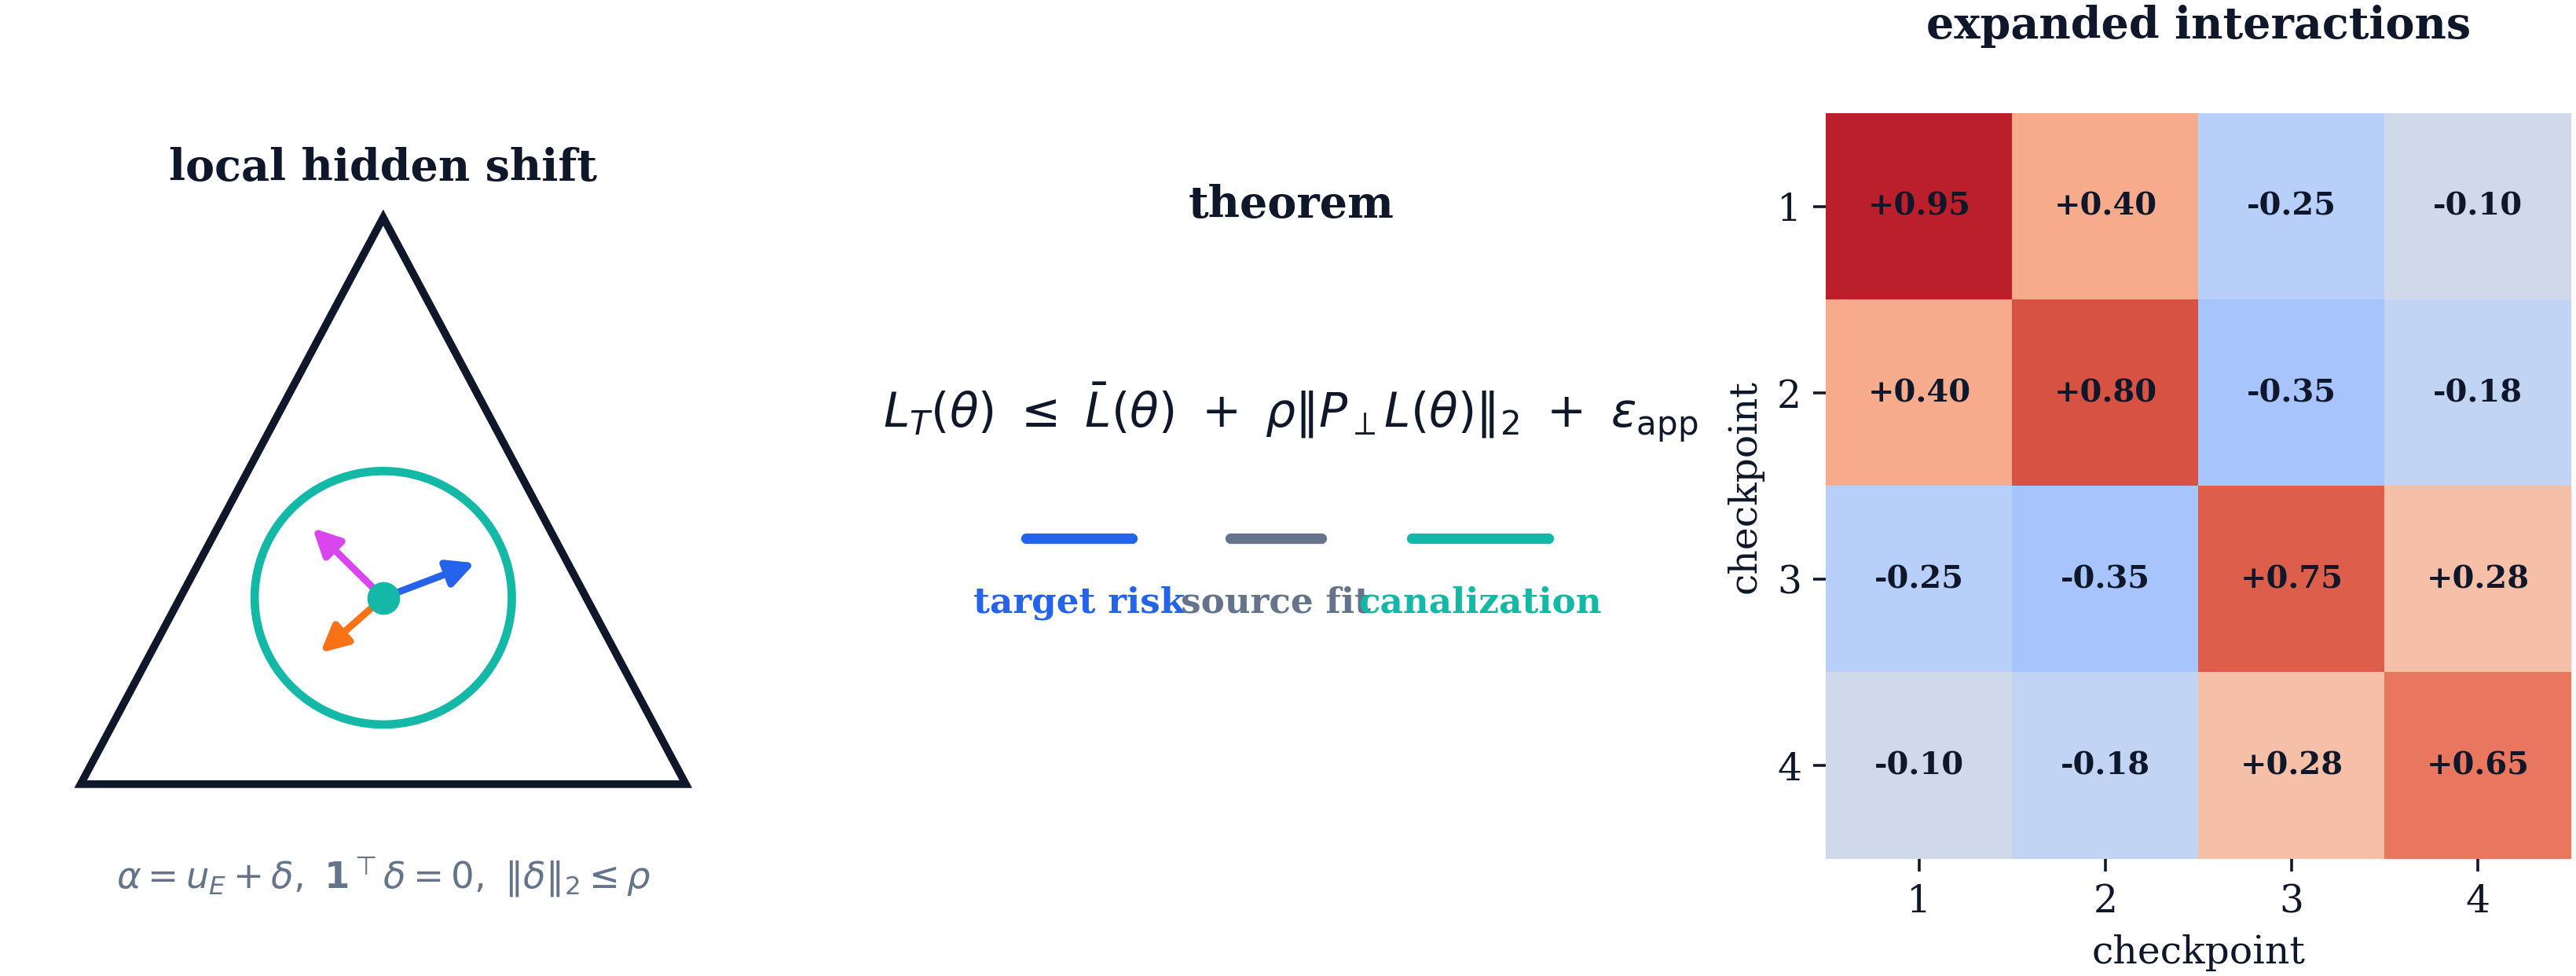
\includegraphics[width=\linewidth]{figures/cda_surrogate_panels.png}
    \caption{\textbf{Canalization decomposes into fit, sensitivity, and interaction.} Left: local source-mixture ambiguity over domain weights. Middle: the exact sensitivity term becomes a centered norm. Right: under a local affine response model, that norm induces pairwise interactions between checkpoints, revealing redundancy and complementarity.}
    \label{fig:surrogate}
\end{figure}

\subsection{Why flatness can help under this larger theory}

\begin{theorem}[Low-curvature aligned neighborhoods imply canalization]
\label{thm:flatness_corollary}
Let \(\theta\in\RR^p\) and \(r>0\). Assume each \(L_e\) is twice continuously differentiable on the ball \(B(\theta,r)\), with
\[
\sup_{\vartheta \in B(\theta,r)} \norm{\nabla^2 L_e(\vartheta)}_{\mathrm{op}} \le H_e.
\]
Then for any \(\theta' \in B(\theta,r)\),
\begin{equation}
\norm{P_\perp L(\theta')}_2
\le
\norm{P_\perp L(\theta)}_2
+ r \norm{P_\perp G(\theta)}_F
+ \frac{r^2}{2}\sqrt{E}\max_{e} H_e,
\label{eq:flatness_bound}
\end{equation}
where \(G(\theta)\in\RR^{E\times p}\) has \(e\)-th row \(\nabla L_e(\theta)^\top\).
\end{theorem}

Theorem~\ref{thm:flatness_corollary} is the precise sense in which flatness can help here. If domain losses are already aligned and local curvature is small, then hidden-shift sensitivity remains small throughout the neighborhood. Flatness is therefore a sufficient low-sensitivity regime. It is not the only one.

\begin{theorem}[Constructive separation from pooled flatness]
\label{thm:separation}
Fix any positive definite matrix \(H\in\RR^{p\times p}\), any \(c>0\), any \(\epsilon \in (0,c)\), and \(E=2\). There exist two candidate minima \(A\) and \(B\) with source-domain losses
\begin{align}
L_1^{A}(\delta)&=c+\frac{1}{2}\delta^\top H \delta, &
L_2^{A}(\delta)&=c+\frac{1}{2}\delta^\top H \delta, \nonumber\\
L_1^{B}(\delta)&=c+\epsilon+\frac{1}{2}\delta^\top H \delta, &
L_2^{B}(\delta)&=c-\epsilon+\frac{1}{2}\delta^\top H \delta,
\label{eq:separation_losses}
\end{align}
such that at \(\delta=0\):
\begin{enumerate}[leftmargin=1.3em]
    \item the pooled loss is identical for \(A\) and \(B\);
    \item the pooled Hessian is identical for \(A\) and \(B\);
    \item for every \(\rho>0\),
    \[
    \mathcal R_\rho(A)=c,
    \qquad
    \mathcal R_\rho(B)=c+\rho\sqrt{2}\,\epsilon.
    \]
\end{enumerate}
Hence any selector based only on pooled loss and pooled local flatness treats \(A\) and \(B\) as equivalent, while distributional canalization strictly prefers \(A\).
\end{theorem}

Theorem~\ref{thm:separation} is an illustrative counterexample showing that pooled flatness need not identify hidden-shift sensitivity.

\begin{figure}[t]
    \centering
    \begin{subfigure}[t]{0.49\linewidth}
        \centering
        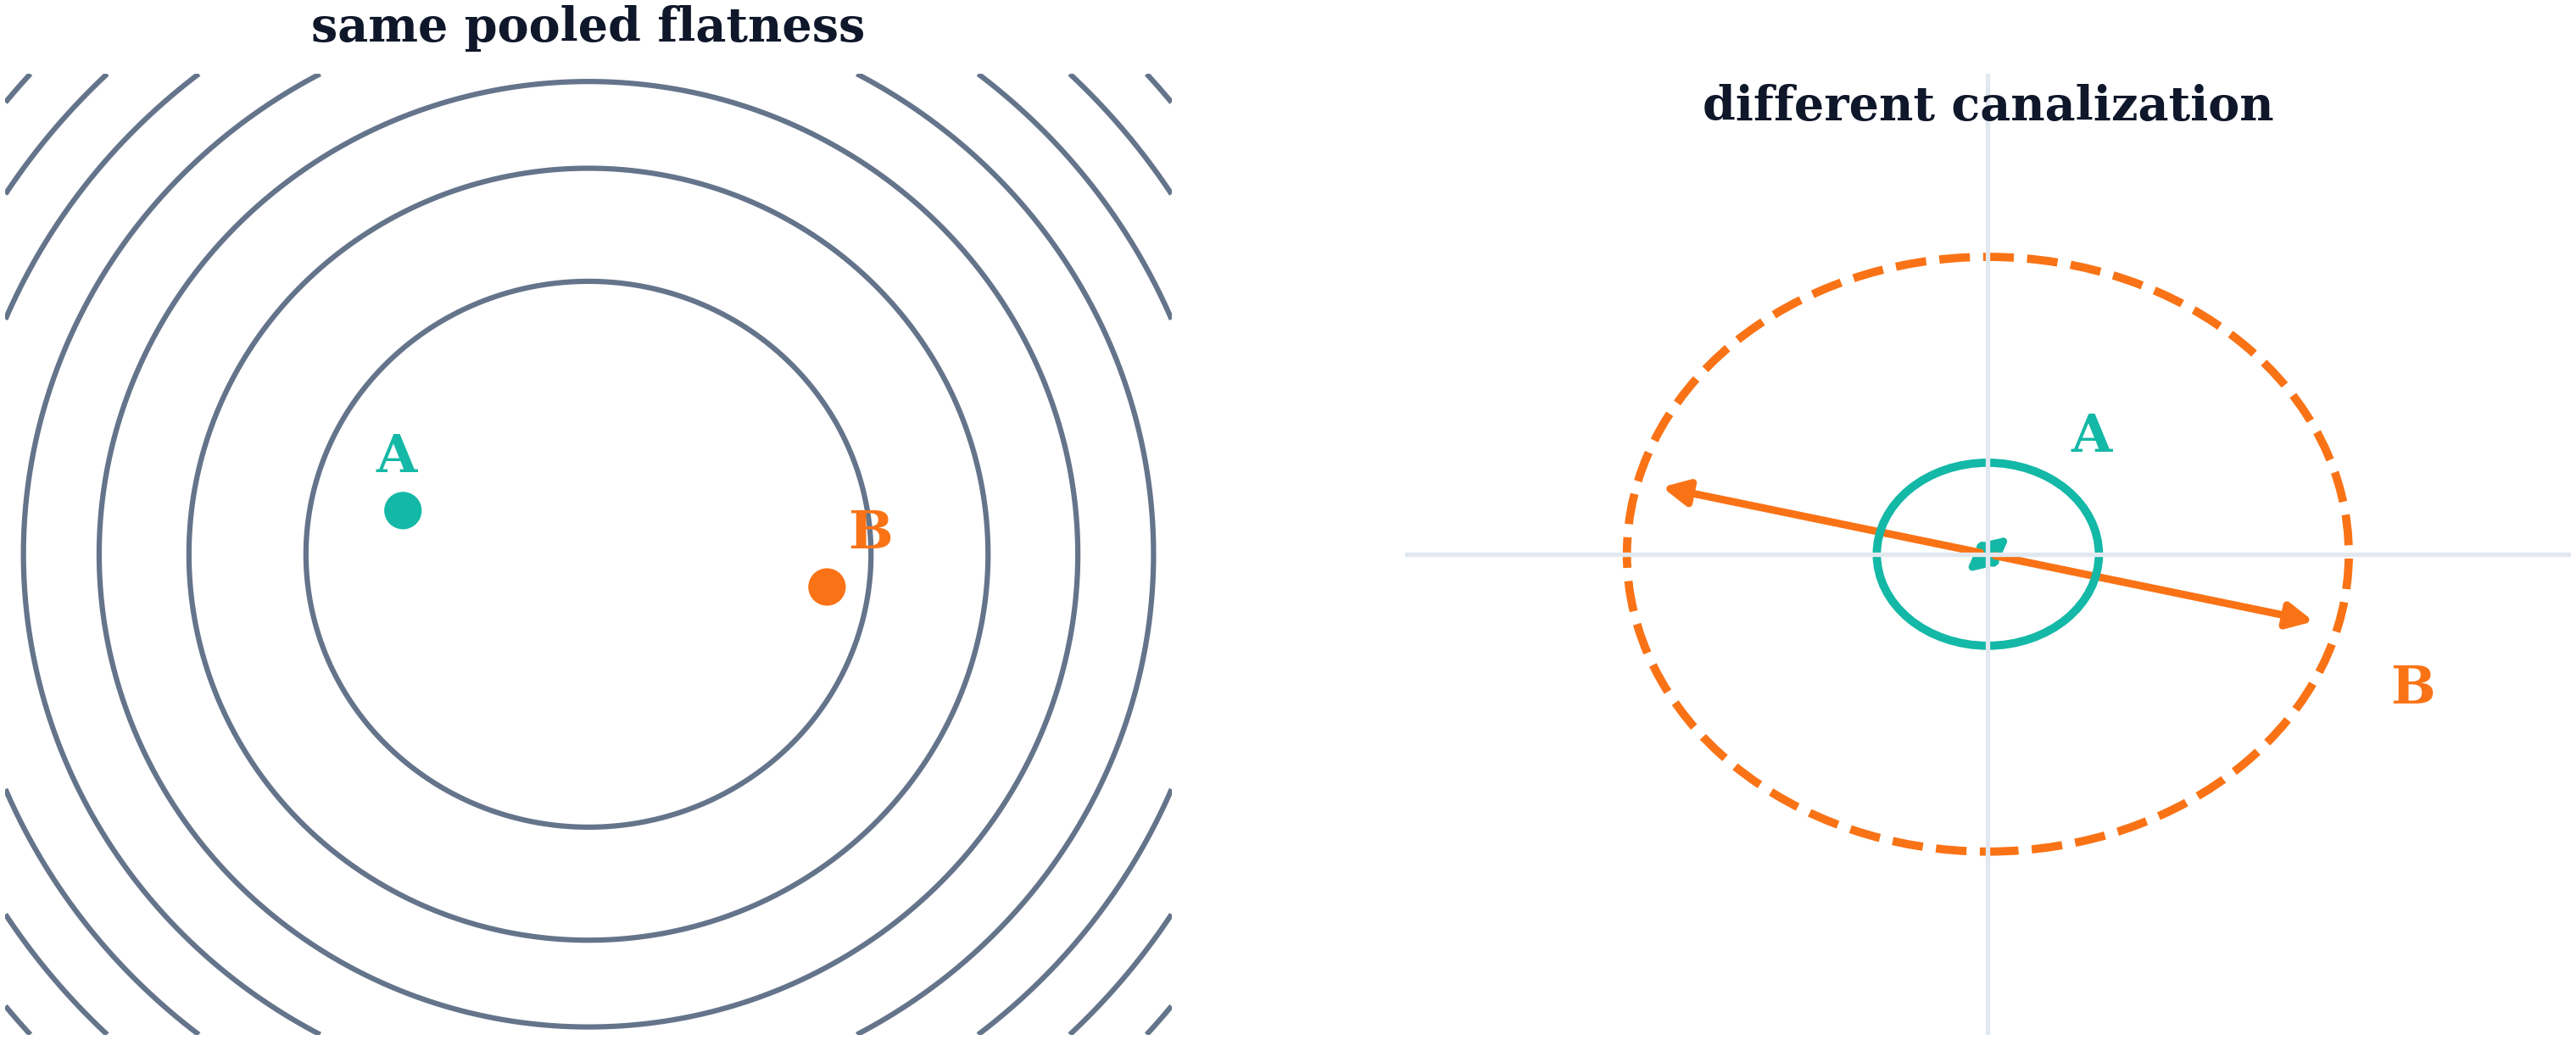
\includegraphics[width=\linewidth]{figures/cda_flatness_vs_canalization.png}
    \end{subfigure}
    \hfill
    \begin{subfigure}[t]{0.49\linewidth}
        \centering
        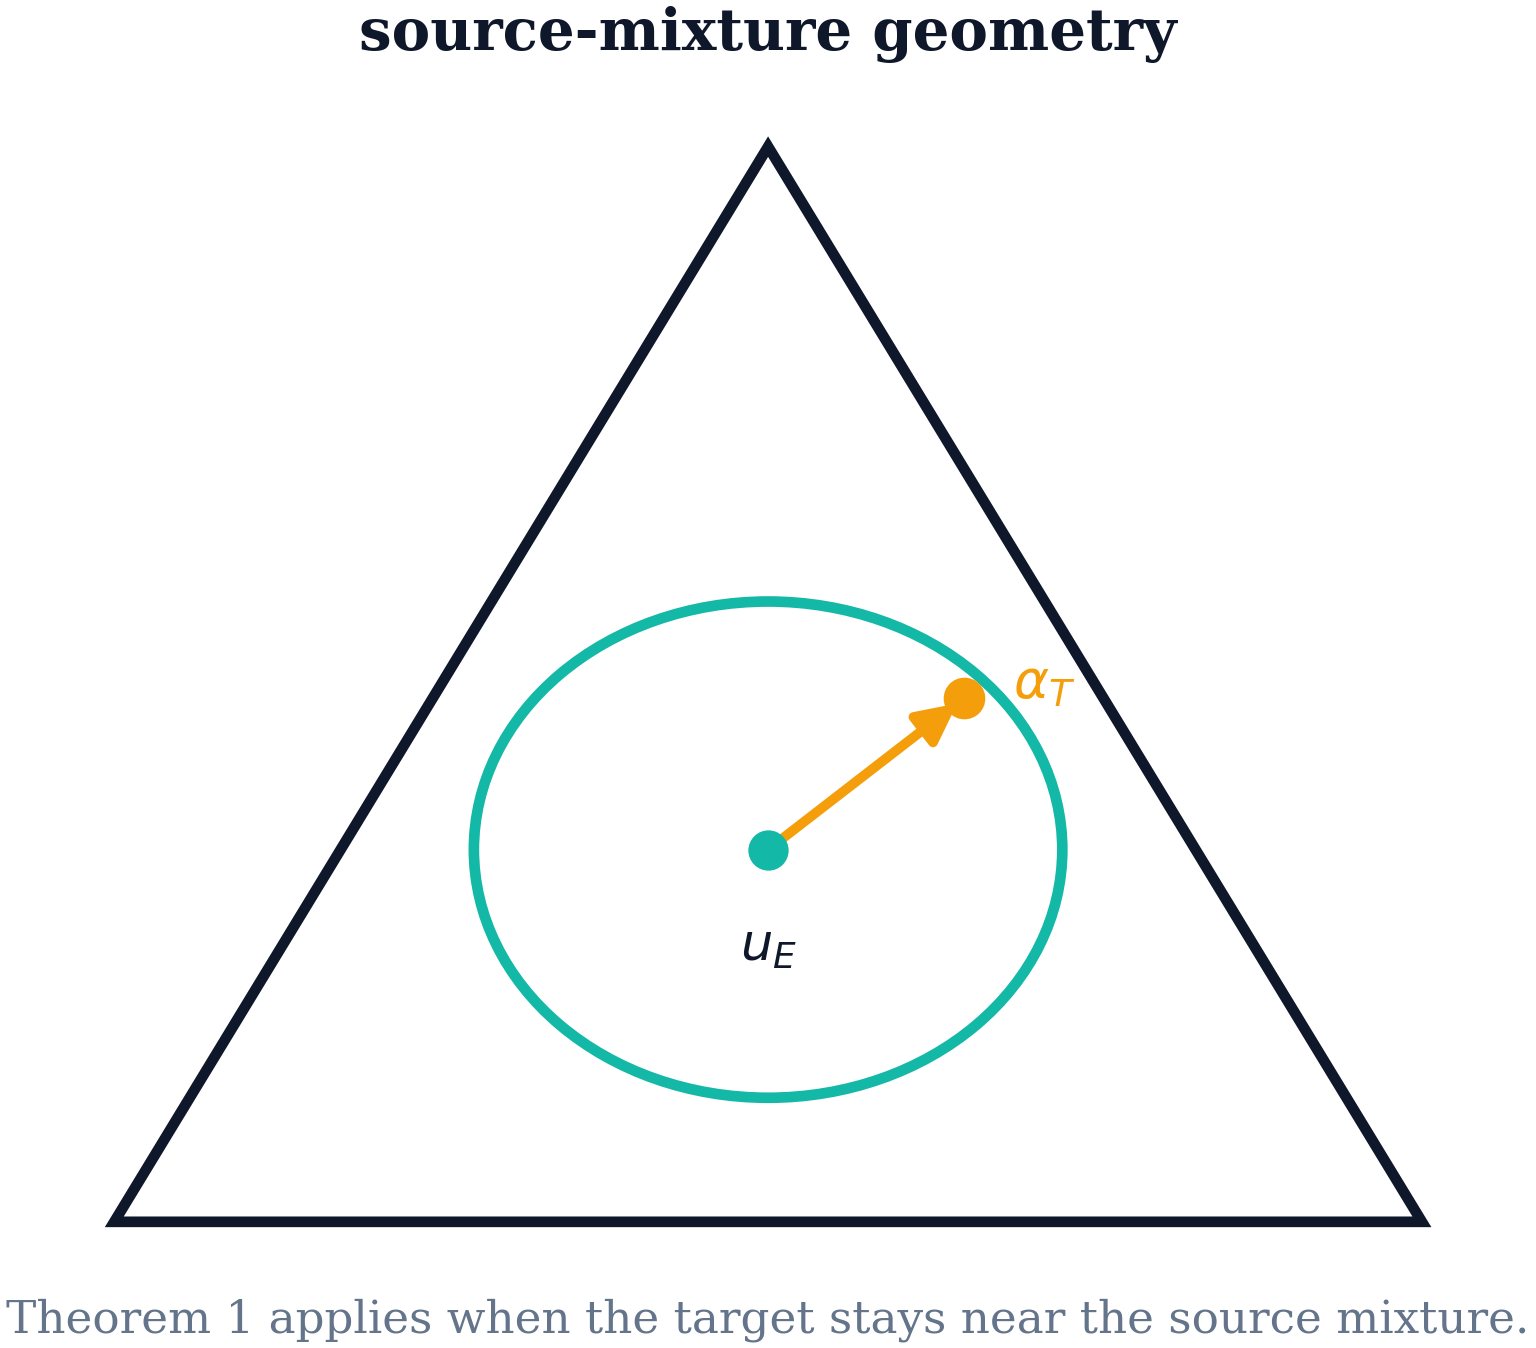
\includegraphics[width=\linewidth]{figures/cda_hidden_shift_simplex.png}
    \end{subfigure}
    \caption{\textbf{Why canalization and pooled flatness can disagree.} Left: two minima can have the same pooled curvature while differing in source-mixture sensitivity. Right: the local hidden-shift ambiguity set lives in source-mixture space, not parameter space.}
    \label{fig:principle}
\end{figure}

\section{Canalized Domain Averaging}
\label{sec:method}

\subsection{Checkpoint bank and theorem-aligned objective}

Let the full checkpoint bank be
\[
\Theta_K = \braces{\theta_t}_{t=1}^{K}.
\]
For theory we first consider an arbitrary retained family
\[
\cC \subseteq \braces{1,\dots,K},
\]
with simplex weights \(w \in \simplex^{|\cC|}\). The deployed soup is
\[
\thetaw = \sum_{t\in\cC} w_t \theta_t.
\]

For each domain \(e\) and validation example \(z_{e,j}=(x_{e,j},y_{e,j})\), define the true-class probability predicted by checkpoint \(t\):
\[
q_{e,j,t} = p_{\theta_t}(y_{e,j}\mid x_{e,j}) \in (0,1].
\]
The predictive-mixture loss on source domain \(e\) is
\begin{equation}
\widehat L_e^{\mathrm{ens}}(w)
=
\frac{1}{n_e}\sum_{j=1}^{n_e}
-\log\paren{\sum_{t\in\cC} w_t q_{e,j,t}}.
\label{eq:ens_loss}
\end{equation}
Collect these losses into
\[
\widehat L^{\mathrm{ens}}(w)
=
\paren{
\widehat L_1^{\mathrm{ens}}(w),
\dots,
\widehat L_E^{\mathrm{ens}}(w)
}^\top.
\]

The theorem-aligned fixed-family objective suggested by Theorem~\ref{thm:target_control} is
\begin{equation}
\Psi_{\mathrm{ens}}(w)
:=
\bar{\widehat L}^{\mathrm{ens}}(w)
+ \lambda_{\mathrm{can}}\norm{P_\perp \widehat L^{\mathrm{ens}}(w)}_2
+ \lambda_{\mathrm{mg}} M(w),
\label{eq:theorem_aligned_family}
\end{equation}
where
\[
\bar{\widehat L}^{\mathrm{ens}}(w)
:=
\frac{1}{E}\one^\top \widehat L^{\mathrm{ens}}(w),
\]
where \(M(w)\) is a mergeability remainder controlling the gap between the predictive mixture and the actual weight soup:
\begin{equation}
M(w)
:=
\max_{e}
\abs{
\widehat L_e(\thetaw)-\widehat L_e^{\mathrm{ens}}(w)
}.
\label{eq:mergeability}
\end{equation}

Equation~\eqref{eq:theorem_aligned_family} is the direct checkpoint-family analogue of the model-level target-risk bound: source fit plus canalization, with mergeability added because one deployable soup must ultimately replace the predictive mixture.

\subsection{From the theorem-aligned objective to \cda{}}

The exact family objective in Eq.~\eqref{eq:theorem_aligned_family} is already the right model-level quantity, but it is inconvenient computationally for two separate reasons. First, the mean-risk term can underweight a badly failing source domain even when Theorem~\ref{thm:target_control} is driven by the hidden-shift envelope. Second, the canalization norm is nonlinear and does not directly expose the interaction structure inside a checkpoint family. The practical algorithm therefore keeps the theorem's \emph{content} but changes its \emph{parameterization}: it strengthens source fit from mean risk to worst-domain risk and upper-bounds the canalization term by a quadratic surrogate on the family.

We first formalize the local affine approximation that makes the interaction structure explicit.

\begin{assumption}[Local affine response model]
\label{ass:affine}
On the retained family \(\cC\), there exist \(b\in\RR^E\) and \(A\in\RR^{E\times |\cC|}\) such that
\[
\widehat L^{\mathrm{ens}}(w)=b+Aw+r(w),
\qquad
\norm{r(w)}_2 \le \epsilon_{\mathrm{aff}}
\]
for all \(w\in\simplex^{|\cC|}\).
\end{assumption}

Under Assumption~\ref{ass:affine}, Proposition~\ref{prop:interaction} identifies the exact quadratic form of the squared canalization penalty on the affine proxy. The next theorem is the formal bridge from the theorem-bearing objective to the practical surrogate.

\begin{theorem}[Quadratic surrogate upper bound]
\label{thm:surrogate_upper}
Let \(K=A^\top P_\perp A\succeq 0\), \(q=A^\top P_\perp b\), and \(c=\norm{P_\perp b}_2^2\) as in Proposition~\ref{prop:interaction}. Under Assumption~\ref{ass:affine}, for every \(\eta>0\) and every \(w\in\simplex^{|\cC|}\),
\begin{equation}
\Psi_{\mathrm{ens}}(w)
\le
\max_{e}\widehat L_e^{\mathrm{ens}}(w)
\;+\;
\frac{\lambda_{\mathrm{can}}}{2\eta}\Bigl(w^\top K w + 2 q^\top w + c\Bigr)
\;+\;
\lambda_{\mathrm{mg}} M(w)
\;+\;
\lambda_{\mathrm{can}}\Bigl(\epsilon_{\mathrm{aff}} + \frac{\eta}{2}\Bigr).
\label{eq:surrogate_upper}
\end{equation}
\end{theorem}

Theorem~\ref{thm:surrogate_upper} is the paper's second main mathematical step. It shows that the practical family-level objective is not an arbitrary mishmash of terms. It comes from three exact or controlled relaxations of the target-risk criterion:
\begin{enumerate}[leftmargin=1.3em]
    \item \(\bar{\widehat L}^{\mathrm{ens}}(w)\le \max_e \widehat L_e^{\mathrm{ens}}(w)\), which turns mean source fit into a robust-source surrogate;
    \item \(\sqrt{x}\le x/(2\eta)+\eta/2\), which converts the canalization norm into a quadratic interaction form;
    \item Assumption~\ref{ass:affine}, which makes the interaction matrix explicit up to \(\epsilon_{\mathrm{aff}}\).
\end{enumerate}
The only additional practical ingredient is mergeability: \(M(w)\) is not computed exactly, so the implementation replaces it with a proxy.

The operational method therefore estimates a positive semidefinite interaction matrix \(C\approx K\), replaces the exact mergeability remainder by a tractable nonnegative proxy \(m^\top w\), and adds a small entropy regularizer to stabilize optimization. This yields the practical \cda{} objective
\begin{equation}
J(w)
:=
\max_{e}\widehat L_e^{\mathrm{ens}}(w)
+ \lambda_{\mathrm{can}} w^\top C w
+ \lambda_{\mathrm{mg}} m^\top w
+ \lambda_{\mathrm{ent}}\sum_{t\in\cC} w_t \log w_t,
\label{eq:practical_objective}
\end{equation}
with \(w\in\simplex^{|\cC|}\).

The first term is the robust-source fit inherited from Proposition~\ref{prop:worst_domain_prior}. The second term is the quadratic hidden-shift surrogate inherited from Theorem~\ref{thm:surrogate_upper}. The third term approximates the mergeability remainder. The entropy term is purely algorithmic. In this sense, \cda{} is exactly the paper's second claim: it is the practical algorithm obtained by expanding and relaxing the target-risk criterion of Theorem~\ref{thm:target_control}.

\subsection{Operational family construction for the surrogate}
\label{subsec:family}

The theorem-bearing criterion is not tied to any particular retained family. The practical surrogate still needs one. In the current instantiation, \cda{} uses a worst-domain anchor and a barrier filter:
\begin{align}
a &\in \argmin_{1\le t\le K} \max_e \widehat L_e(\theta_t),
\label{eq:anchor}\\
\cC
&=
\braces{
t :
\max_e \widehat L_e(\theta_t) \le \max_e \widehat L_e(\theta_a)+\epsilon,
\;
B(t,a)\le \tau
},
\label{eq:family}
\end{align}
where \(B(t,a)\) is a line-interpolation barrier between checkpoint \(t\) and anchor \(a\). This stage is an operational heuristic justified by mergeability. It is not the source of the main theoretical claim.

\begin{algorithm}[t]
\caption{\cda{} on a checkpoint bank}
\label{alg:cda}
\begin{algorithmic}[1]
\Require dense checkpoint bank \(\Theta_K=\{\theta_t\}_{t=1}^{K}\), held-out source validation splits \(\{\cV_e\}_{e=1}^{E}\), family thresholds \((\epsilon,\tau)\), objective weights \((\lambda_{\mathrm{can}},\lambda_{\mathrm{mg}},\lambda_{\mathrm{ent}})\)
\State \(a \gets \argmin_{1\le t\le K}\max_e \widehat L_e(\theta_t)\)
\State \(\cC \gets \{t:\max_e \widehat L_e(\theta_t)\le \max_e \widehat L_e(\theta_a)+\epsilon,\; B(t,a)\le\tau\}\)
\ForAll{\(t\in\cC\)}
    \State Cache \(q_{e,j,t}=p_{\theta_t}(y_{e,j}\mid x_{e,j})\) for all \((e,j)\)
\EndFor
\State Form \(\widehat L_e^{\mathrm{ens}}(w)\) by Eq.~\eqref{eq:ens_loss}
\State Form \(C\succeq 0\) and \(m\in\RR_{\ge 0}^{|\cC|}\)
\State \(w^\star \gets \argmin_{w\in\simplex^{|\cC|}} J(w)\) by projected subgradient descent or mirror descent
\State \(\bar\theta \gets \sum_{t\in\cC} w_t^\star \theta_t\)
\State Refresh BN statistics and return \(\bar\theta\)
\end{algorithmic}
\end{algorithm}

\begin{figure}[t]
    \centering
    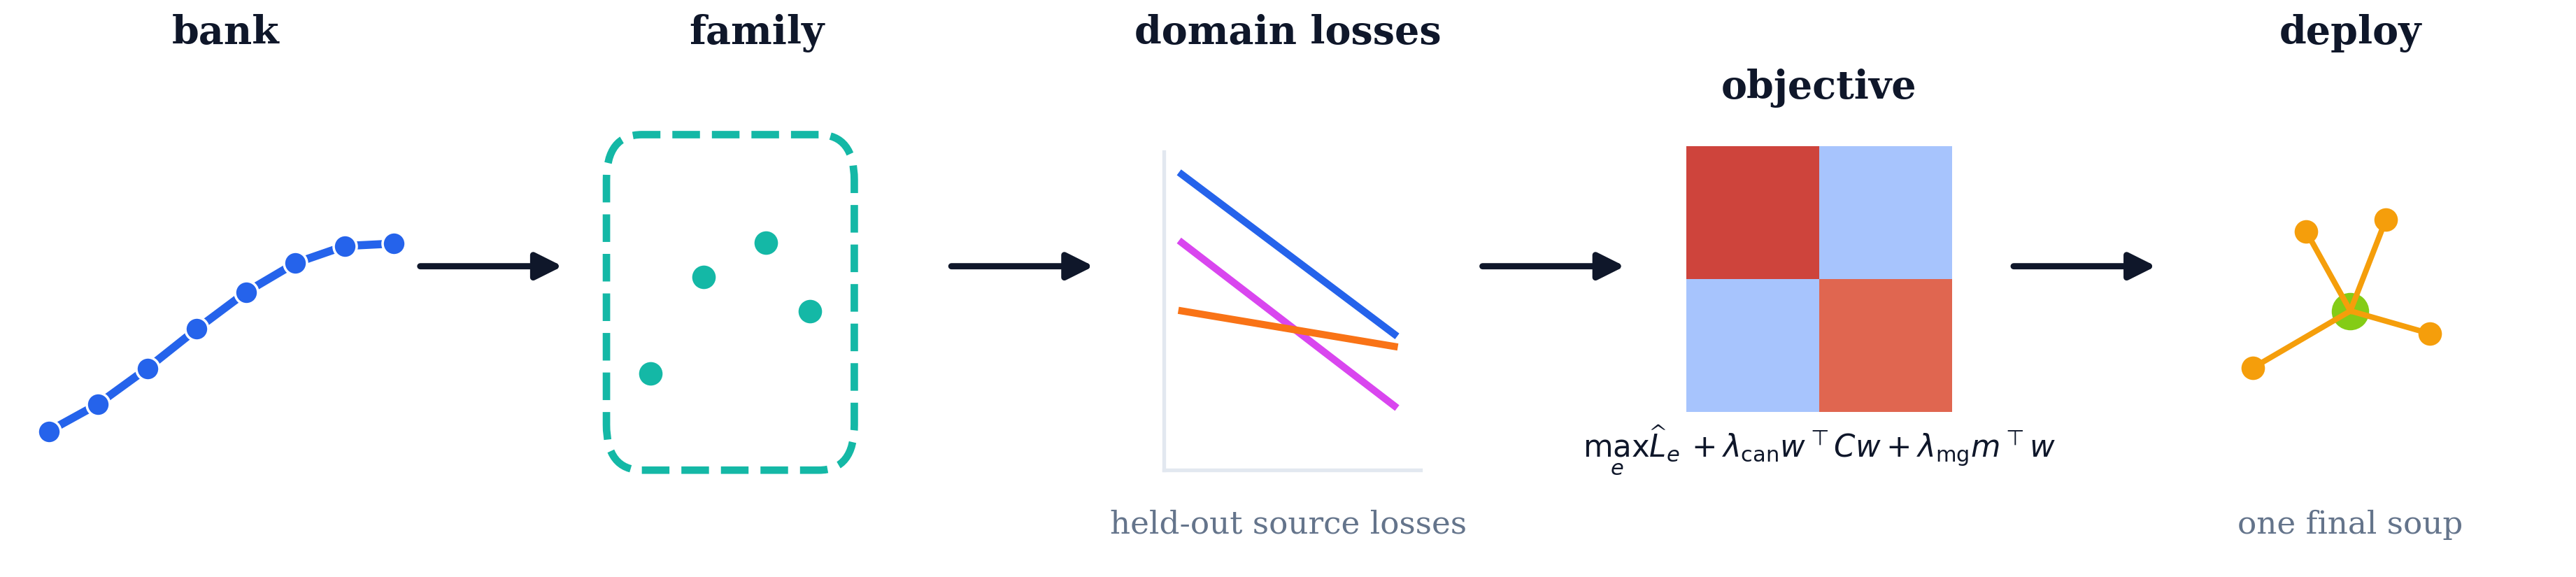
\includegraphics[width=\linewidth]{figures/cda_method_panels.png}
    \caption{\textbf{What the practical \cda{} pipeline is doing.} Every panel here is operational rather than theorem-bearing. The bank is first restricted by a heuristic mergeability screen. The optimizer then chooses weights to reduce worst-domain source loss while suppressing an interaction-based surrogate of hidden-shift sensitivity. The final output is still one deployable soup, and the predictive-mixture-to-soup bridge is controlled only conditionally through mergeability.}
    \label{fig:method}
\end{figure}

\section{Theory for the Practical Objective}
\label{sec:theory}

\subsection{Convexity and optimization}

\begin{proposition}[Convexity]
\label{prop:convexity}
Assume each \(w\mapsto \widehat L_e^{\mathrm{ens}}(w)\) is convex on \(\simplex^{|\cC|}\), \(C \succeq 0\), \(\lambda_{\mathrm{can}}\ge 0\), and \(\lambda_{\mathrm{ent}}\ge 0\). Then \(J\) in Eq.~\eqref{eq:practical_objective} is convex on \(\simplex^{|\cC|}\).
\end{proposition}

\begin{theorem}[Projected-subgradient convergence]
\label{thm:convergence}
Let \(D=\sqrt{2}\) denote the diameter of the simplex in \(\ell_2\). Assume every subgradient of \(J\) on \(\simplex^{|\cC|}\) has norm at most \(G\). Let \(\{w_t\}_{t=1}^{T}\) be generated by projected subgradient descent
\[
w_{t+1}=\proj_{\simplex}\paren{w_t-\eta_t g_t},
\qquad
g_t \in \partial J(w_t),
\qquad
\eta_t=\frac{D}{G\sqrt{t}}.
\]
Then the \(\eta_t\)-weighted averaged iterate
\[
\tilde w_T
:=
\frac{\sum_{t=1}^{T}\eta_t w_t}{\sum_{t=1}^{T}\eta_t}
\]
satisfies
\begin{equation}
J(\tilde w_T)-\min_{w\in\simplex^{|\cC|}} J(w)
\le
\frac{DG(2+\log T)}{2\sqrt{T}}.
\label{eq:psg_rate}
\end{equation}
\end{theorem}

\subsection{Exact control of the deployed soup is conditional}

The exact identities above control the predictive mixture. The deployed object is the actual weight-space soup. That transfer requires a separate mergeability assumption.

\begin{assumption}[Mergeability remainder]
\label{ass:mergeability}
There exists a nonnegative function \(R(w)\) such that for all \(w\in\simplex^{|\cC|}\),
\begin{equation}
\norm{
\widehat L(\thetaw)-\widehat L^{\mathrm{ens}}(w)
}_\infty
\le
R(w),
\label{eq:mergeability_assumption}
\end{equation}
where \(\widehat L(\thetaw)=\paren{\widehat L_1(\thetaw),\dots,\widehat L_E(\thetaw)}^\top\).
\end{assumption}

\begin{theorem}[Predictive-mixture-to-single-soup transfer]
\label{thm:transfer}
Under Assumption~\ref{ass:mergeability}, for any \(w\in\simplex^{|\cC|}\),
\begin{equation}
\max_e \widehat L_e(\thetaw)
\le
\max_e \widehat L_e^{\mathrm{ens}}(w) + R(w),
\label{eq:max_transfer}
\end{equation}
and
\begin{equation}
\norm{P_\perp \widehat L(\thetaw)}_2
\le
\norm{P_\perp \widehat L^{\mathrm{ens}}(w)}_2 + \sqrt{E}\,R(w).
\label{eq:canal_transfer}
\end{equation}
Consequently, for any \(\lambda_{\mathrm{can}}\ge 0\),
\begin{equation}
\max_e \widehat L_e(\thetaw)
+ \lambda_{\mathrm{can}}\norm{P_\perp \widehat L(\thetaw)}_2
\le
\max_e \widehat L_e^{\mathrm{ens}}(w)
+ \lambda_{\mathrm{can}}\norm{P_\perp \widehat L^{\mathrm{ens}}(w)}_2
+ (1+\lambda_{\mathrm{can}}\sqrt{E})R(w).
\label{eq:objective_transfer}
\end{equation}
\end{theorem}

Theorem~\ref{thm:transfer} is the main caveat of the paper. All exact guarantees are stated for the predictive-mixture objective on a fixed retained family. The transfer to one deployed soup is conditional, approximate, and controlled entirely by the mergeability remainder.

\subsection{Why exact weights can matter less than support discovery}

\begin{theorem}[Low-curvature face bound]
\label{thm:face}
Assume \(J\) is twice differentiable on a face \(F\) of the simplex containing \(w^\star\), with Hessian restricted to \(F\) bounded by
\[
0 \preceq \nabla^2 J(w)\vert_F \preceq \mu I
\qquad
\text{for all } w\in F.
\]
Assume also that \(w^\star\) is first-order stationary on the affine hull of \(F\), i.e. \(\nabla_F J(w^\star)=0\).
Then for any \(w \in F\),
\begin{equation}
J(w)-J(w^\star)
\le
\frac{\mu}{2}\norm{w-w^\star}_2^2.
\label{eq:face_bound}
\end{equation}
In particular, if a broad face of the simplex has small curvature, then many weight vectors on that face achieve nearly the same objective value.
\end{theorem}

Theorem~\ref{thm:face} explains why exact optimized weights can matter less than finding the right interacting support. Once the optimizer identifies a low-curvature complementary face, uniform-on-support weights may already be near-optimal.

\begin{figure}[t]
    \centering
    \begin{subfigure}[t]{0.49\linewidth}
        \centering
        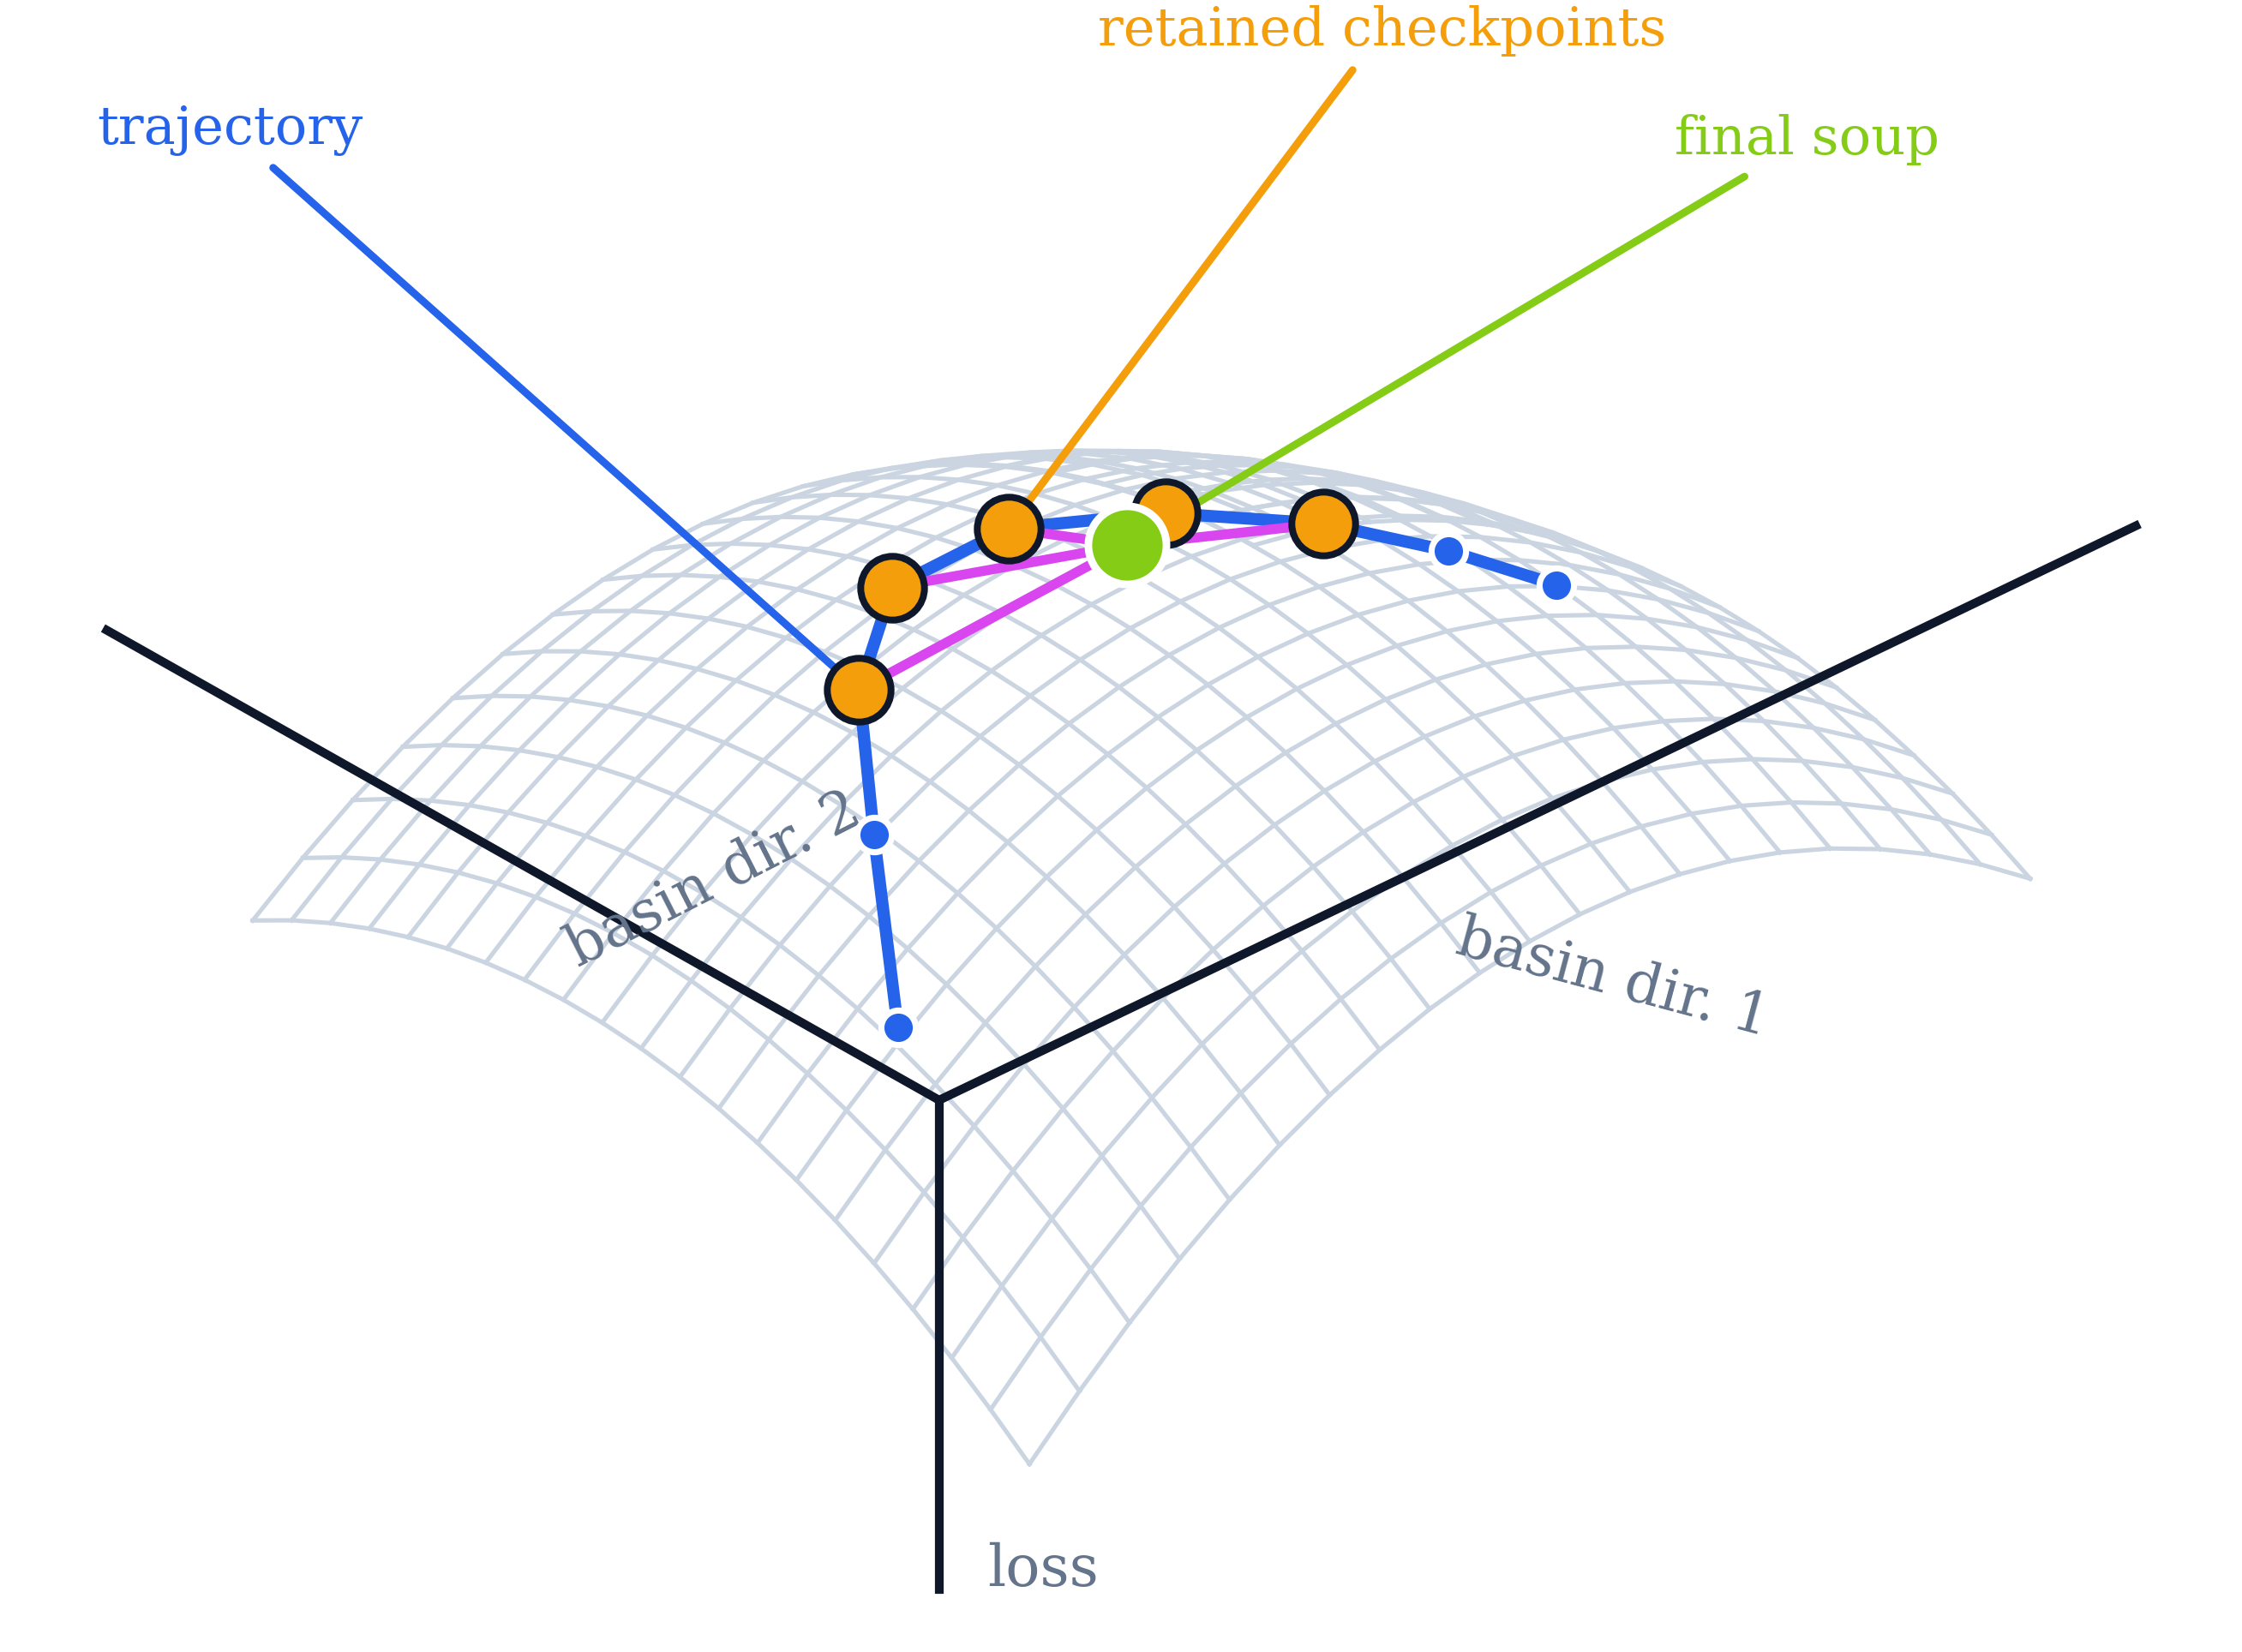
\includegraphics[width=\linewidth]{figures/cda_3d_basin.png}
    \end{subfigure}
    \hfill
    \begin{subfigure}[t]{0.49\linewidth}
        \centering
        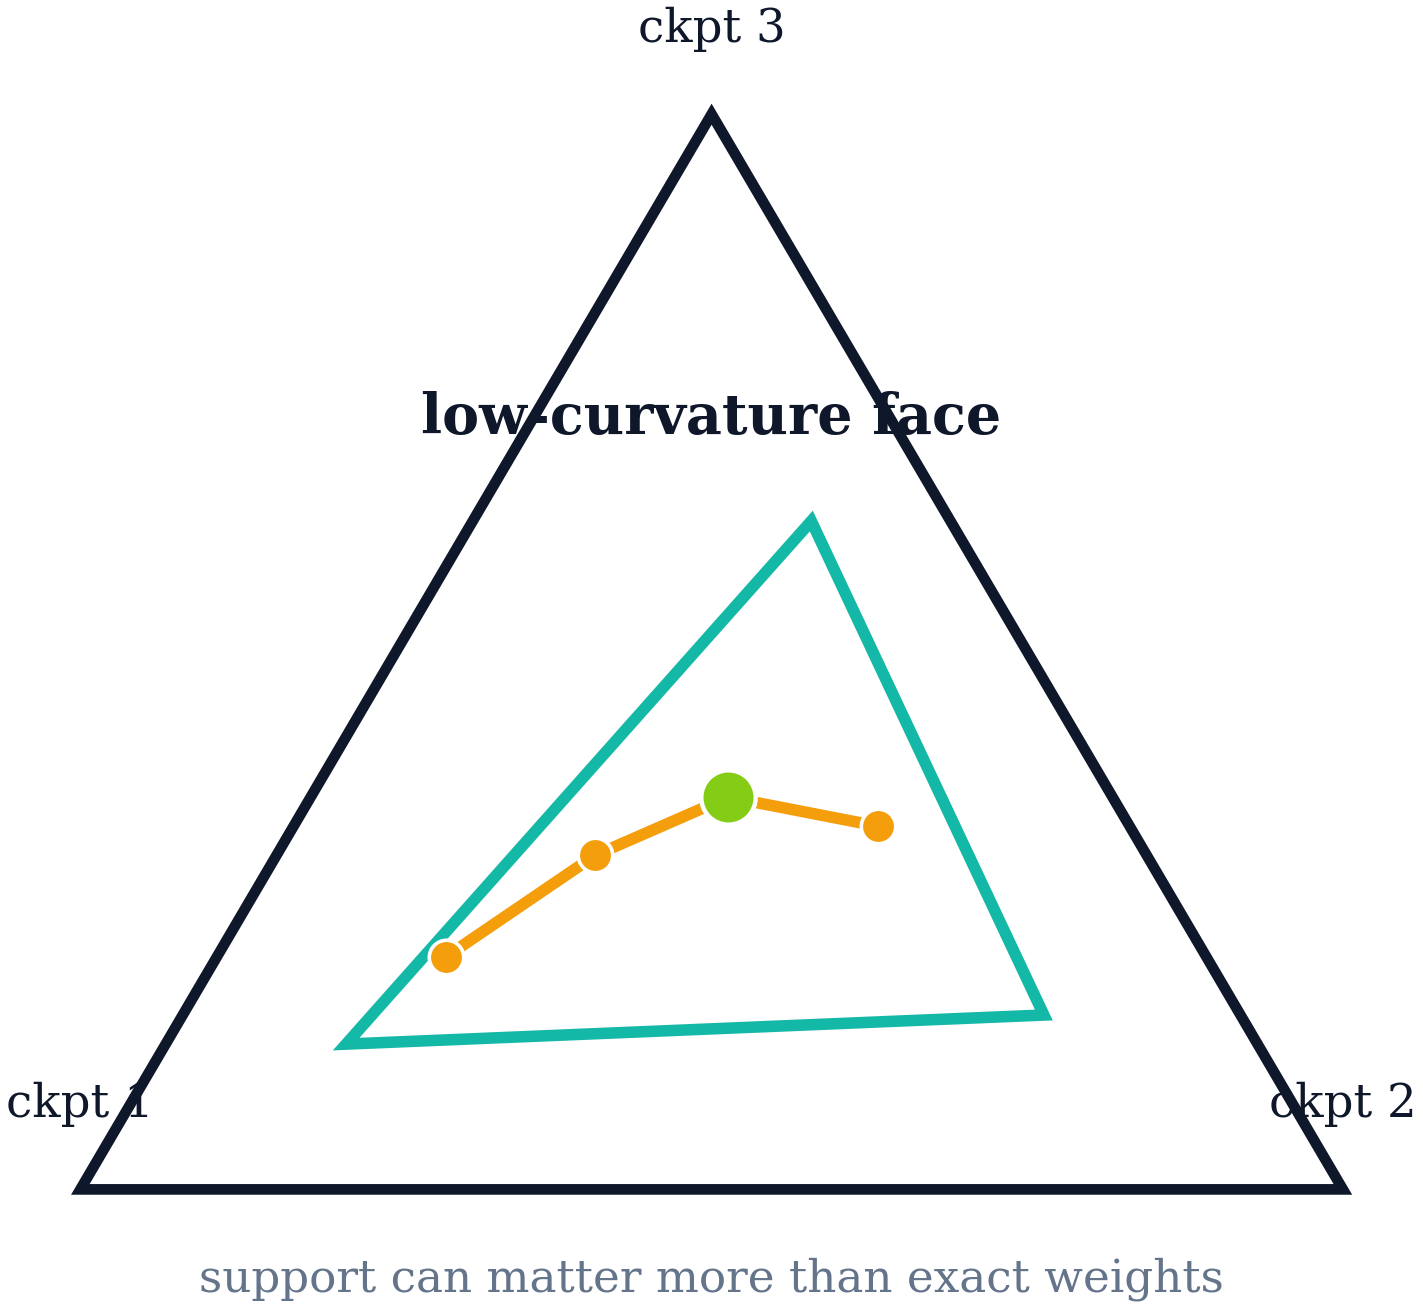
\includegraphics[width=\linewidth]{figures/cda_simplex_face.png}
    \end{subfigure}
    \caption{\textbf{Mergeability and support discovery.} Left: a corner-view illustration of a locally mergeable region inside a checkpoint bank. Right: once a complementary face of the simplex is found, objective curvature can be low enough that exact weights matter less than the support itself.}
    \label{fig:3d}
\end{figure}

\section{Empirical Evaluation}
\label{sec:experiments}

\subsection{Evaluation protocol}

The intended experimental protocol follows the standard DomainBed-style DG setting used by recent post-hoc DG papers. The main benchmark suite consists of PACS, VLCS, OfficeHome, TerraIncognita, and DomainNet. Each environment is held out in turn as the target domain. A single ERM training run with an ImageNet-pretrained ResNet-50 backbone produces the checkpoint bank, and the post-hoc method is then allowed to access only source-domain held-out splits. The final reported metric is out-of-domain classification accuracy on the held-out target domain, with per-domain numbers and a dataset average.

The post-hoc inputs required by \cda{} are:
\begin{itemize}[leftmargin=1.3em]
    \item one dense trajectory checkpoint bank from the completed ERM run;
    \item held-out source-domain validation splits for estimating domain losses;
    \item no target examples, no retraining, and one final deployable soup.
\end{itemize}
The minimum ablation suite required to identify the theory is:
\begin{itemize}[leftmargin=1.3em]
    \item remove the canalization term while keeping family construction fixed;
    \item replace worst-domain risk with pooled source fit;
    \item remove the mergeability term;
    \item replace optimized simplex weights with uniform-on-support weights;
    \item hold the surrogate objective fixed while varying the retained family.
\end{itemize}

\subsection{Published benchmark context}

Table~\ref{tab:published_context} records exact published reference points that define the empirical bar. The table is intentionally limited to numbers that were verified from the paper sources already present in the workspace.

\begin{table}[t]
    \centering
    \caption{\textbf{Published benchmark context from prior post-hoc DG papers.} These are exact published numbers, copied from the cited sources. They are reference context, not direct head-to-head reruns under a single codebase.}
    \label{tab:published_context}
    \begin{tabular}{lcccccc}
        \toprule
        Method & PACS & VLCS & OfficeHome & TerraInc. & DomainNet & Avg. \\
        \midrule
        \erm{} \citep{cha2021swad} & 85.5 & 77.5 & 66.5 & 46.1 & 40.9 & 63.3 \\
        \swad{} \citep{cha2021swad} & 88.1 & 79.1 & 70.6 & 50.0 & 46.5 & 66.9 \\
        \eoa{} \citep{arpit2021ensemble} & 87.7 & 78.5 & 69.1 & 48.8 & 46.1 & 66.0 \\
        \diwa{}\(^{\dagger}\) \citep{rame2022diwa} & 89.0 & 78.6 & 72.8 & 51.9 & 47.7 & 68.0 \\
        \bottomrule
    \end{tabular}
\end{table}

For PACS, the published per-domain values are especially useful because they expose the regime in which current post-hoc methods are already strong.

\begin{table}[t]
    \centering
    \caption{\textbf{Published PACS domain-wise context.} Values are exact published out-of-domain accuracies from the cited papers.}
    \label{tab:pacs_context}
    \begin{tabular}{lccccc}
        \toprule
        Method & Art & Cartoon & Photo & Sketch & Avg. \\
        \midrule
        \swad{} \citep{cha2021swad} & 89.3 & 83.4 & 97.3 & 82.5 & 88.1 \\
        \diwa{}\(^{\dagger}\) \citep{rame2022diwa} & 90.6 & 83.4 & 98.2 & 83.8 & 89.0 \\
        \bottomrule
    \end{tabular}
\end{table}

\subsection{Manuscript replacement tables}

The next three tables are \emph{not measured results}. They are manuscript-layout placeholders so the full paper structure is complete before the remaining runs finish. Every gray italic value is an expected replacement value and must be overwritten by real measurements before submission.

\begin{table}[t]
    \centering
    \caption{\textbf{Expected full-benchmark table for final replacement.} Gray italic values are placeholders, not empirical claims.}
    \label{tab:expected_main}
    \begin{tabular}{lcccccc}
        \toprule
        Method & PACS & VLCS & OfficeHome & TerraInc. & DomainNet & Avg. \\
        \midrule
        \erm{} & 85.5 & 77.5 & 66.5 & 46.1 & 40.9 & 63.3 \\
        \swad{} & 88.1 & 79.1 & 70.6 & 50.0 & 46.5 & 66.9 \\
        \diwa{}\(^{\dagger}\) & 89.0 & 78.6 & 72.8 & 51.9 & 47.7 & 68.0 \\
        \cda{} & \Expected{89.3} & \Expected{79.7} & \Expected{73.4} & \Expected{52.5} & \Expected{48.2} & \Expected{68.6} \\
        \bottomrule
    \end{tabular}
\end{table}

\begin{table}[t]
    \centering
    \caption{\textbf{Expected PACS domain-wise table for final replacement.} Gray italic values are placeholders, not empirical claims.}
    \label{tab:expected_pacs}
    \begin{tabular}{lccccc}
        \toprule
        Method & Art & Cartoon & Photo & Sketch & Avg. \\
        \midrule
        \swad{} & 89.3 & 83.4 & 97.3 & 82.5 & 88.1 \\
        \diwa{}\(^{\dagger}\) & 90.6 & 83.4 & 98.2 & 83.8 & 89.0 \\
        \cda{} & \Expected{90.1} & \Expected{84.7} & \Expected{98.0} & \Expected{84.5} & \Expected{89.3} \\
        \bottomrule
    \end{tabular}
\end{table}

\begin{table}[t]
    \centering
    \caption{\textbf{Expected ablation table for final replacement.} Gray italic values are placeholders, not empirical claims.}
    \label{tab:expected_ablation}
    \begin{tabular}{lc}
        \toprule
        Variant & PACS Avg. \\
        \midrule
        \cda{} full & \Expected{89.3} \\
        w/o canalization term & \Expected{88.5} \\
        w/o mergeability term & \Expected{88.1} \\
        pooled-fit instead of worst-domain fit & \Expected{88.4} \\
        uniform-on-support soup & \Expected{88.9} \\
        \bottomrule
    \end{tabular}
\end{table}

\subsection{What would count as evidence for the theory}

The theory is not confirmed merely by beating a baseline once. The theory would be empirically supported only if four things happen simultaneously:
\begin{enumerate}[leftmargin=1.3em]
    \item the full method improves target accuracy over strong post-hoc baselines;
    \item removing the canalization term materially hurts performance while holding the family fixed;
    \item worst-domain fit plus canalization outperforms pooled source fit alone;
    \item the predictive-mixture optimizer transfers to a single soup with a small mergeability remainder.
\end{enumerate}
If gains disappear under those ablations, then the paper's main story would collapse back to generic checkpoint selection or generic flat-region averaging.

\section{Discussion}
\label{sec:discussion}

\paragraph{Why this is beyond flatness.}
The central theorem of the paper is not a flatness theorem. It is a hidden-shift theorem in source-mixture space. Flatness enters only through Theorem~\ref{thm:flatness_corollary}, where low curvature and domain-gradient alignment imply small source-mixture sensitivity. In that sense, flatness is one sufficient mechanism for canalization, not the defining object itself.

\paragraph{Why complementarity appears automatically.}
The interaction matrix in Proposition~\ref{prop:interaction} is not hand-designed. It appears because the canalization norm is squared and expanded on a checkpoint family. Negative or weak off-diagonal interactions correspond to checkpoints whose domain-response profiles cancel rather than reinforce each other. This is the formal reason the practical method can prefer noncontiguous but complementary soups.

\paragraph{Why mergeability must remain explicit.}
The theory is exact for the model-level criterion and for predictive mixtures on a fixed family. It does not become exact for a single deployed soup without Theorem~\ref{thm:transfer}. This is why mergeability is not a cosmetic engineering add-on. It is the term that prevents the practical method from optimizing a good predictive mixture that fails when materialized in weight space.

\paragraph{What would falsify the paper's thesis.}
The paper would be materially weakened by any of the following outcomes: the canalization term has no effect after family construction is controlled; the practical objective wins only because of the retained family heuristic; or the predictive-mixture optimum does not transfer to a real soup. These are not edge cases. They are the main empirical risks.

\section{Limitations}

This paper has four important limitations.
\begin{enumerate}[leftmargin=1.3em]
    \item The exact hidden-shift identity is exact for the centered \(\ell_2\) tangent perturbation model around the source mixture and the domain-loss vector. It is not an unconditional target-shift certificate.
    \item Theorem~\ref{thm:target_control} is conditional on the source-supported hidden-shift assumption. If the target domain lies far outside the local source-mixture hull, the guarantee does not apply.
    \item The practical \cda{} objective is a surrogate: it uses a retained family, a quadratic interaction approximation, and a mergeability proxy. Those steps are controlled but not exact.
    \item The gray italic values in Tables~\ref{tab:expected_main}--\ref{tab:expected_ablation} are manuscript placeholders for later replacement. They are included only to complete the paper structure before the final benchmark runs are finished.
\end{enumerate}

\section{Conclusion}

This paper is organized around two claims.

First, we propose a model-level objective beyond flatness: minima with low sensitivity to small redistributions of source-support mass are more generalizable under a source-supported hidden-shift model. This is Theorem~\ref{thm:target_control}. The exact hidden-shift identity of Proposition~\ref{prop:exact_identity}, the variance and interaction decompositions of Propositions~\ref{prop:variance_form} and \ref{prop:interaction}, and the flatness corollary of Theorem~\ref{thm:flatness_corollary} together explain why source-mixture sensitivity is the broader object and why flatness can still work as one special regime.

Second, we develop a practical post-hoc checkpoint-soup algorithm by expanding and relaxing that objective. Theorem~\ref{thm:surrogate_upper} shows how the exact canalization objective turns into a robust-source fit term, a quadratic interaction term, and a mergeability term, which together lead to \cda{}. In this view, the practical algorithm is not the theory itself. It is the family-level surrogate implied by the theory.

The empirical part of the manuscript is intentionally split into verified published context and clearly marked replacement tables. That separation is deliberate. The mathematical contribution should stand on its own, and the final experimental claim should only be made after the remaining benchmark runs are complete.

\appendix

\section{Proofs}

\subsection{Proof of Theorem~\ref{thm:target_control}}

\begin{proof}
Under Assumption~\ref{ass:source_supported}, there exists \(\alpha_T\in \cA_\rho\) such that
\[
L_T(\theta)\le \alpha_T^\top L(\theta)+\epsilon_{\mathrm{app}}.
\]
Since \(\alpha_T\in \cA_\rho\), its value under the linear functional \(\alpha\mapsto \alpha^\top L(\theta)\) is bounded by the supremum over \(\cA_\rho\). Hence
\[
L_T(\theta)
\le
\sup_{\alpha\in\cA_\rho}\alpha^\top L(\theta)+\epsilon_{\mathrm{app}}
=
\mathcal R_\rho(\theta)+\epsilon_{\mathrm{app}},
\]
which proves Eq.~\eqref{eq:target_control_abstract}. Substituting Proposition~\ref{prop:exact_identity} into Eq.~\eqref{eq:target_control_abstract} gives Eq.~\eqref{eq:target_control_explicit}.
\end{proof}

\subsection{Proof of Proposition~\ref{prop:exact_identity}}

\begin{proof}
By definition of the tangent ambiguity set \(\cA_\rho\), we may write \(\alpha=\ub+\delta\), where \(\one^\top\delta=0\) and \(\norm{\delta}_2\le \rho\). Then
\[
\alpha^\top L(\theta)
=
\ub^\top L(\theta) + \delta^\top L(\theta)
=
\bar L(\theta) + \delta^\top P_\perp L(\theta),
\]
because \(\delta^\top \one=0\). By Cauchy--Schwarz,
\[
\delta^\top P_\perp L(\theta)
\le
\norm{\delta}_2 \norm{P_\perp L(\theta)}_2
\le
\rho \norm{P_\perp L(\theta)}_2.
\]
If \(P_\perp L(\theta)\neq 0\), equality is achieved by
\[
\delta^\star
=
\rho \frac{P_\perp L(\theta)}{\norm{P_\perp L(\theta)}_2},
\]
which satisfies \(\one^\top\delta^\star=0\). If \(P_\perp L(\theta)=0\), both sides are zero. Therefore
\[
\sup_{\alpha\in\cA_\rho}\alpha^\top L(\theta)
=
\bar L(\theta) + \rho \norm{P_\perp L(\theta)}_2.
\]
\end{proof}

\subsection{Proof of Proposition~\ref{prop:worst_domain_prior}}

\begin{proof}
The objective \(\pi \mapsto \pi^\top L(\theta)\) is linear on the simplex \(\simplex^E\). A linear function on a simplex attains its maximum at an extreme point. The extreme points are the standard basis vectors \(e_1,\dots,e_E\), so
\[
\sup_{\pi\in\simplex^E} \pi^\top L(\theta)
=
\max_{1\le e\le E} e_e^\top L(\theta)
=
\max_{1\le e\le E}L_e(\theta).
\]
\end{proof}

\subsection{Proof of Proposition~\ref{prop:variance_form}}

\begin{proof}
Because \(P_\perp L=L-\bar L\one\),
\[
\norm{P_\perp L}_2^2
=
\sum_{e=1}^{E}(L_e-\bar L)^2.
\]
Also,
\[
\Var_{e\sim \ub}(L_e)
=
\frac{1}{E}\sum_{e=1}^{E}(L_e-\bar L)^2,
\]
which implies Eq.~\eqref{eq:variance_form}.
\end{proof}

\subsection{Proof of Proposition~\ref{prop:interaction}}

\begin{proof}
Under the affine proxy,
\[
\norm{P_\perp(b+Aw)}_2^2
=
(b+Aw)^\top P_\perp (b+Aw)
=
w^\top A^\top P_\perp A w + 2 w^\top A^\top P_\perp b + b^\top P_\perp b.
\]
This is Eq.~\eqref{eq:quadratic_canalization}. Writing \(a_t=P_\perp A_{\cdot t}\), we have
\[
Aw = \sum_t w_t A_{\cdot t},
\qquad
P_\perp Aw = \sum_t w_t a_t,
\]
so
\[
w^\top K w
=
\norm{\sum_t w_t a_t}_2^2
=
\sum_t w_t^2 \norm{a_t}_2^2
+ 2\sum_{s<t} w_s w_t \inner{a_s}{a_t}.
\]
\end{proof}

\subsection{Proof of Theorem~\ref{thm:surrogate_upper}}

\begin{proof}
Fix \(w\in\simplex^{|\cC|}\). By definition,
\[
\Psi_{\mathrm{ens}}(w)
=
\bar{\widehat L}^{\mathrm{ens}}(w)
+
\lambda_{\mathrm{can}}\norm{P_\perp \widehat L^{\mathrm{ens}}(w)}_2
+
\lambda_{\mathrm{mg}} M(w).
\]
Since the mean is bounded by the maximum coordinate,
\[
\bar{\widehat L}^{\mathrm{ens}}(w)
\le
\max_e \widehat L_e^{\mathrm{ens}}(w).
\]
Under Assumption~\ref{ass:affine},
\[
\widehat L^{\mathrm{ens}}(w)=b+Aw+r(w),
\qquad
\norm{r(w)}_2\le \epsilon_{\mathrm{aff}}.
\]
Therefore
\[
\norm{P_\perp \widehat L^{\mathrm{ens}}(w)}_2
\le
\norm{P_\perp(b+Aw)}_2 + \norm{P_\perp r(w)}_2
\le
\norm{P_\perp(b+Aw)}_2 + \epsilon_{\mathrm{aff}}.
\]
By Proposition~\ref{prop:interaction},
\[
\norm{P_\perp(b+Aw)}_2^2
=
w^\top K w + 2 q^\top w + c.
\]
Now apply the scalar inequality
\[
\sqrt{x}\le \frac{x}{2\eta}+\frac{\eta}{2}
\qquad
\text{for all } x\ge 0,\; \eta>0
\]
with \(x=w^\top K w + 2 q^\top w + c\). This gives
\[
\norm{P_\perp(b+Aw)}_2
\le
\frac{1}{2\eta}\Bigl(w^\top K w + 2 q^\top w + c\Bigr)+\frac{\eta}{2}.
\]
Combining the previous three displays yields
\[
\norm{P_\perp \widehat L^{\mathrm{ens}}(w)}_2
\le
\frac{1}{2\eta}\Bigl(w^\top K w + 2 q^\top w + c\Bigr)
+
\epsilon_{\mathrm{aff}}
+
\frac{\eta}{2}.
\]
Multiplying by \(\lambda_{\mathrm{can}}\), adding the bound on \(\bar{\widehat L}^{\mathrm{ens}}(w)\), and keeping \(\lambda_{\mathrm{mg}}M(w)\) unchanged proves Eq.~\eqref{eq:surrogate_upper}.
\end{proof}

\subsection{Proof of Theorem~\ref{thm:flatness_corollary}}

\begin{proof}
Fix \(\theta' \in B(\theta,r)\) and write \(\Delta=\theta'-\theta\). For each domain \(e\), Taylor's theorem with integral remainder gives
\[
L_e(\theta')
=
L_e(\theta)
+ \inner{\nabla L_e(\theta)}{\Delta}
+ \int_{0}^{1}(1-s)\Delta^\top \nabla^2 L_e(\theta+s\Delta)\Delta \, ds.
\]
Collecting these equations across domains yields
\[
L(\theta')
=
L(\theta) + G(\theta)\Delta + h(\Delta),
\]
where the \(e\)-th coordinate of \(h(\Delta)\) is the integral remainder above. By the Hessian bound,
\[
\abs{h_e(\Delta)}
\le
\frac{1}{2}H_e \norm{\Delta}_2^2
\le
\frac{1}{2}\max_e H_e \, r^2.
\]
Therefore
\[
\norm{h(\Delta)}_2
\le
\frac{1}{2}\sqrt{E}\max_e H_e \, r^2.
\]
Apply \(P_\perp\) and the triangle inequality:
\[
\norm{P_\perp L(\theta')}_2
\le
\norm{P_\perp L(\theta)}_2
+ \norm{P_\perp G(\theta)\Delta}_2
+ \norm{P_\perp h(\Delta)}_2.
\]
Now
\[
\norm{P_\perp G(\theta)\Delta}_2
\le
\norm{P_\perp G(\theta)}_F \norm{\Delta}_2
\le
r \norm{P_\perp G(\theta)}_F,
\]
and
\[
\norm{P_\perp h(\Delta)}_2 \le \norm{h(\Delta)}_2
\le
\frac{1}{2}\sqrt{E}\max_e H_e \, r^2.
\]
Combining the bounds proves Eq.~\eqref{eq:flatness_bound}.
\end{proof}

\subsection{Proof of Theorem~\ref{thm:separation}}

\begin{proof}
At \(\delta=0\), we have
\[
L_1^A(0)=L_2^A(0)=c,
\qquad
L_1^B(0)=c+\epsilon,
\quad
L_2^B(0)=c-\epsilon.
\]
Hence the pooled source loss is
\[
\frac{L_1^A(0)+L_2^A(0)}{2}=c
=
\frac{L_1^B(0)+L_2^B(0)}{2}.
\]
The pooled Hessian of both candidates is
\[
\frac{1}{2}\nabla^2 L_1^A(0)+\frac{1}{2}\nabla^2 L_2^A(0)
=
H
=
\frac{1}{2}\nabla^2 L_1^B(0)+\frac{1}{2}\nabla^2 L_2^B(0).
\]
Thus any pooled-flatness selector that uses only the pooled loss and pooled Hessian cannot distinguish them.

For \(A\), the domain-loss vector is \(L^A(0)=(c,c)\), so \(P_\perp L^A(0)=0\). By Proposition~\ref{prop:exact_identity},
\[
\mathcal R_\rho(A)=c.
\]
For \(B\),
\[
L^B(0)=\begin{pmatrix} c+\epsilon \\ c-\epsilon \end{pmatrix},
\qquad
\bar L^B(0)=c,
\qquad
P_\perp L^B(0)=\begin{pmatrix} \epsilon \\ -\epsilon \end{pmatrix}.
\]
Therefore
\[
\norm{P_\perp L^B(0)}_2=\sqrt{2}\,\epsilon,
\]
and Proposition~\ref{prop:exact_identity} gives
\[
\mathcal R_\rho(B)=c+\rho\sqrt{2}\,\epsilon.
\]
\end{proof}

\subsection{Proof of Proposition~\ref{prop:convexity}}

\begin{proof}
For fixed \(e,j\), the map
\[
w \mapsto -\log\paren{\sum_{t\in\cC} w_t q_{e,j,t}}
\]
is convex on the simplex because it is the composition of a linear map and the convex decreasing function \(-\log\) on \((0,\infty)\). Averaging over \(j\) preserves convexity, so each \(\widehat L_e^{\mathrm{ens}}(w)\) is convex. The pointwise maximum over \(e\) is convex. Since \(C\succeq 0\), the quadratic term \(w^\top C w\) is convex. The linear term \(m^\top w\) is convex. Finally, \(x\mapsto x\log x\) is convex on \([0,\infty)\), so the entropy term is convex. The sum of convex functions is convex.
\end{proof}

\subsection{Proof of Theorem~\ref{thm:convergence}}

\begin{proof}
This is the standard projected-subgradient bound on a convex set of diameter \(D\). For completeness, we record the main steps. Let \(w^\star\) be an optimizer. Nonexpansiveness of Euclidean projection implies
\[
\norm{w_{t+1}-w^\star}_2^2
\le
\norm{w_t-\eta_t g_t-w^\star}_2^2
=
\norm{w_t-w^\star}_2^2
-2\eta_t \inner{g_t}{w_t-w^\star}
+ \eta_t^2 \norm{g_t}_2^2.
\]
By the subgradient inequality,
\[
J(w_t)-J(w^\star)\le \inner{g_t}{w_t-w^\star}.
\]
Rearranging,
\[
2\eta_t \paren{J(w_t)-J(w^\star)}
\le
\norm{w_t-w^\star}_2^2
-\norm{w_{t+1}-w^\star}_2^2
+\eta_t^2 G^2.
\]
Summing from \(t=1\) to \(T\) and using \(\norm{w_1-w^\star}_2\le D\) gives
\[
\sum_{t=1}^{T} \eta_t \paren{J(w_t)-J(w^\star)}
\le
\frac{D^2}{2}
+ \frac{G^2}{2}\sum_{t=1}^{T}\eta_t^2.
\]
With \(\eta_t=D/(G\sqrt t)\), we have
\[
\sum_{t=1}^{T}\eta_t \ge \frac{D}{G}\sqrt T,
\qquad
\sum_{t=1}^{T}\eta_t^2 \le \frac{D^2}{G^2}(1+\log T).
\]
By convexity,
\[
J\!\paren{\frac{\sum_{t=1}^{T}\eta_t w_t}{\sum_{t=1}^{T}\eta_t}}
\le
\frac{\sum_{t=1}^{T}\eta_t J(w_t)}{\sum_{t=1}^{T}\eta_t}.
\]
Therefore
\[
J(\tilde w_T)-J(w^\star)
\le
\frac{\frac{D^2}{2}+\frac{G^2}{2}\sum_{t=1}^{T}\eta_t^2}{\sum_{t=1}^{T}\eta_t}.
\]
Using the bounds in Eq.~\eqref{eq:psg_rate} gives
\[
J(\tilde w_T)-J(w^\star)
\le
\frac{\frac{D^2}{2}+\frac{D^2}{2}(1+\log T)}{(D/G)\sqrt{T}}
=
\frac{DG(2+\log T)}{2\sqrt{T}},
\]
which proves Eq.~\eqref{eq:psg_rate}.
\end{proof}

\subsection{Proof of Theorem~\ref{thm:transfer}}

\begin{proof}
Eq.~\eqref{eq:max_transfer} follows immediately from Assumption~\ref{ass:mergeability}:
\[
\widehat L_e(\thetaw) \le \widehat L_e^{\mathrm{ens}}(w)+R(w)
\qquad
\text{for all } e,
\]
so taking the maximum over \(e\) yields Eq.~\eqref{eq:max_transfer}.

For Eq.~\eqref{eq:canal_transfer}, write
\[
P_\perp \widehat L(\thetaw)
=
P_\perp \widehat L^{\mathrm{ens}}(w)
+ P_\perp\paren{\widehat L(\thetaw)-\widehat L^{\mathrm{ens}}(w)}.
\]
By the triangle inequality,
\[
\norm{P_\perp \widehat L(\thetaw)}_2
\le
\norm{P_\perp \widehat L^{\mathrm{ens}}(w)}_2
+ \norm{P_\perp\paren{\widehat L(\thetaw)-\widehat L^{\mathrm{ens}}(w)}}_2.
\]
The second term is bounded by the \(\ell_2\) norm of a vector whose coordinates are each bounded by \(R(w)\), hence
\[
\norm{P_\perp\paren{\widehat L(\thetaw)-\widehat L^{\mathrm{ens}}(w)}}_2
\le
\sqrt{E}\,R(w).
\]
Combining with Eq.~\eqref{eq:max_transfer} proves Eq.~\eqref{eq:objective_transfer}.
\end{proof}

\subsection{Proof of Theorem~\ref{thm:face}}

\begin{proof}
Restrict \(J\) to the affine hull of face \(F\). Taylor's theorem around \(w^\star\) gives
\[
J(w)
=
J(w^\star)
+ \inner{\nabla J(w^\star)}{w-w^\star}
+ \frac{1}{2}(w-w^\star)^\top \nabla^2 J(\xi)(w-w^\star)
\]
for some \(\xi\) on the line segment between \(w^\star\) and \(w\). Since \(w-w^\star\) lies in the affine hull of \(F\) and \(\nabla_F J(w^\star)=0\), the first-order term vanishes. Using \(\nabla^2 J(\xi)\vert_F \preceq \mu I\) yields
\[
J(w)-J(w^\star)
\le
\frac{\mu}{2}\norm{w-w^\star}_2^2.
\]
\end{proof}

\bibliographystyle{plainnat}
\bibliography{references}

\end{document}
